% ============================================================
%  Chapter 3 — Optical Amplification and Laser Fundamentals
%  Style: student-voice notes matching the personal style guide
% ============================================================

At the close of the previous chapter, we derived the fundamental macroscopic propagation equation for the photon flux $\Phi$, arriving at the compact result $\Phi(z) = \Phi(0)\,e^{\gamma z}$ where $\gamma = \sigma(N_2 - N_1)$ is the gain coefficient. The key insight was that the exponential growth of the field depends entirely on the \emph{sign} of $\gamma$: if $N_2 > N_1$, the medium amplifies; if $N_2 < N_1$, it absorbs. Everything that follows in this chapter is really an answer to one question: \emph{how do we engineer a real medium to have $N_2 > N_1$, and what are the performance consequences when we do?}

% =============================================================
\section{Population Inversion}
% =============================================================

\subsection{What It Is and Why We Need It}

Population inversion is the condition of a medium in which the upper energy level $E_2$ contains \emph{more} atoms than the lower energy level $E_1$: that is, $N_2 > N_1$. This phenomenon is called inversion because it \textbf{inverts} the natural thermal ordering of the populations. Since $\gamma = \sigma(N_2 - N_1)$, a positive population difference directly makes $\gamma > 0$ — the necessary condition for optical amplification.

The analogy with a water pump is instructive: just as you need a pump to move water from a lower reservoir to a higher one against gravity, you need a \textbf{pump} to move atoms from $E_1$ to $E_2$ against the Boltzmann distribution.

\subsection{The Pumping Mechanism}

The pump must continuously excite atoms from the ground state $E_1$ up to a higher energy level fast enough to maintain $N_2 > N_1$. Crucially, the pump operates on the atomic populations independently of the signal — it is not driven by the light we want to amplify, but by a separate external energy source.

The pump can in principle be any energy source that atoms can absorb: an electron beam whose electrons collide with atoms and donate kinetic energy, or a separate energetic light source at a different frequency.

We characterise the pump generically by its \textbf{pumping rate} $R$, which is the net rate at which atoms are transferred from the ground state $E_1$ up to the upper lasing level $E_2$ per unit volume per unit time (units: atoms~m$^{-3}$~s$^{-1}$).

\subsection{The Metastable State Requirement}

There is one more condition that is absolutely necessary for population inversion to be sustainable: the upper level $E_2$ must be a \textbf{metastable state}. A metastable state is an energy level with an unusually long spontaneous emission lifetime. Why is this so critical?

After the pump has placed atoms in $E_2$, those atoms will eventually decay back down by spontaneous emission. If the lifetime of $E_2$ is very short, atoms will immediately fall back down before stimulated emission from the signal can exploit them, making it impossible to maintain $N_2 > N_1$. If, on the other hand, the lifetime of $E_2$ is very long (metastable), atoms pile up in $E_2$ and stay there long enough to sustain the inversion.

For sustained population inversion, the physical requirements are therefore clear: we need (1) a strong pump to bulldoze atoms upwards from the ground state $E_1$, and (2) the upper level $E_2$ must be metastable.

% =============================================================
\section{The Two-Level Laser --- and Why It Cannot Work}
% =============================================================

Before introducing complex architectures, we must ask: why not directly pump a two-level system? By shining an intense optical pump tuned precisely to the resonant energy gap ($h\nu_0 = E_2 - E_1$), we would intuitively expect to drive the overwhelming majority of ground-state atoms into $E_2$. Let us formally test this hypothesis using the rate equation.

With a pump photon flux density $\Phi_p$ and an interaction cross-section $\sigma$, there are three fundamental processes governing the population $N_2$:
\begin{enumerate}
    \item \textbf{Absorption (Pump Up):} The pump photons excite atoms from $E_1$ to $E_2$ at a rate $+\sigma\Phi_p\,N_1$.
    \item \textbf{Stimulated Emission (Pump Down):} Because the quantum mechanical probabilities for absorption and stimulated emission are precisely identical, the same pump photons will inevitably force atoms in $E_2$ back down to $E_1$ at a rate $-\sigma\Phi_p\,N_2$.
    \item \textbf{Spontaneous Emission (Decay):} Atoms in $E_2$ naturally decay back to $E_1$ governed by their spontaneous lifetime $\tau_{sp}$. This gives a rate $-\frac{N_2}{\tau_{sp}}$.
\end{enumerate}

Combining these independent processes, the complete differential equation describing the rate of change of the upper level population is:
\begin{equation*}
    \frac{dN_2}{dt} = \underbrace{\sigma\Phi_p\,N_1}_{\text{Absorption}} - \underbrace{\sigma\Phi_p\,N_2}_{\text{Stim. Emission}} - \underbrace{\frac{N_2}{\tau_{sp}}}_{\text{Spont. Emission}}
\end{equation*}

\subsection{Steady-State Analysis}

To determine the maximum achievable populations, we let the system settle into steady state where the atomic populations no longer change in time ($dN_2/dt = 0$). Setting the derivative strictly to zero gives:
\begin{equation*}
    0 = \sigma\Phi_p\,N_1 - \sigma\Phi_p\,N_2 - \frac{N_2}{\tau_{sp}}
\end{equation*}

To solve for the population ratio $N_2/N_1$, we formally balance the rates by moving all terms containing $N_2$ to the left-hand side (which physically equates the sum of all downward decay rates to the isolated upward absorption rate):
\begin{equation*}
    \sigma\Phi_p\,N_2 + \frac{N_2}{\tau_{sp}} = \sigma\Phi_p\,N_1
\end{equation*}

Factoring out $N_2$ on the left:
\begin{equation*}
    N_2\!\left(\sigma\Phi_p + \frac{1}{\tau_{sp}}\right) = \sigma\Phi_p\,N_1
\end{equation*}

Finally, dividing both sides by $N_1$ and by the bracketed term gives us our explicit steady-state ratio:
\begin{keyresult}
\begin{equation}
    \frac{N_2}{N_1} = \frac{\sigma\Phi_p}{\sigma\Phi_p + \dfrac{1}{\tau_{sp}}}
\end{equation}
\end{keyresult}

\subsection{The Physical Impossibility of Inversion}

Look closely at the algebraic structure of this result. The numerator is exactly $\sigma\Phi_p$, while the denominator is that same $\sigma\Phi_p$ \emph{plus} a strictly positive constant ($1/\tau_{sp} > 0$). Because the denominator will always mathematically exceed the numerator for any finite pump power, it dictates an absolute ceiling on the populations:
\begin{equation*}
    \frac{N_2}{N_1} < 1 \quad \text{unconditionally.}
\end{equation*}

What happens if we buy the most expensive, infinitely powerful pump laser in the world ($\Phi_p \to \infty$)? As the pump rate completely dominates the finite spontaneous emission term, the $1/\tau_{sp}$ fraction vanishes, and the $\sigma\Phi_p$ terms cancel out. The population ratio asymptotically approaches exactly $1$:
\begin{equation*}
    \lim_{\Phi_p \to \infty} \frac{N_2}{N_1} = 1
\end{equation*}
When $N_1 = N_2$, the medium reaches the \textbf{transparency condition} where the net gain is precisely zero. The intense pump light simply passes through as if the medium weren't there at all, but the population never truly inverts.

\begin{keyinsight}[The Fundamental Flaw of the Two-Level System]
The physical failure here stems directly from Einstein's observation that the coefficients for absorption and stimulated emission are strictly equal ($B_{12} = B_{21}$). The very same optical transition the pump uses to push ground-state atoms \emph{up} is identical to the transition that stimulated emission uses to push excited atoms \emph{back down}. 

As you continuously dial up the pump power, you certainly increase the upward excitation rate, but you symmetrically and inescapably increase the downward stimulated rate. The pump is fundamentally fighting its own success. The system can at best equalise the two populations (transparency), but it can never tip the scales into a true inversion ($N_2 > N_1$). 
\end{keyinsight}

Because a two-level system is perfectly symmetric and self-limiting, optical amplification using only two levels is physically impossible. We are therefore forced to introduce intermediary energy levels (the three-level and four-level architectures) to physically decouple the pumping pathway from the lasing pathway, breaking the mathematical symmetry and allowing an inversion to safely accumulate.

% =============================================================
\section{The Three-Level Laser System and Kinetics}
% =============================================================

By introducing a fast-decaying intermediary energy level, we route atoms through pathways that successfully bypass the two-level failure. In a three-level laser setup, the generic pump exclusively excites atoms from $E_1$ (the ground state) up to a third level $E_3$. Atoms then quickly fall from $E_3$ down to the metastable level $E_2$ via non-radiative emission (releasing heat, not light). Finally, the incoming signal stimulates these trapped atoms to drop from $E_2$ back down to $E_1$. Because the signal and the pump operate on entirely different energy gaps, the signal safely triggers amplification without inadvertently fighting the upward pump.

The fundamental difficulty with a three-level laser is that the lower lasing level \emph{is} the ground state, which is naturally extremely heavily populated. Therefore, a massive optical pump power is required to successfully invert the population, because at least half of the total atoms in the medium must be physically lifted to $E_2$.

The overall pumping rate $R$ can be constant or dynamically driven. If the pump is an optical signal of flux density $\Phi_p$, the rate depends entirely on the available ground state population:
\begin{equation*}
    R = \sigma_p\,\Phi_p\,N_1
\end{equation*}
where $\sigma_p$ is the specific absorption cross-section for the $E_1 \to E_3$ pump transition.

\begin{keyinsight}[Is a Monochromatic Pump Required?]
A logical paradox arises: if pumping requires the exact photon energy ($h\nu_p = E_3 - E_1$), wouldn't the pump itself need to be a perfectly monochromatic laser? If you need a laser to build a laser, how was the first one ever built?

The physical workaround is that $E_3$ is rarely a single, sharp quantum line. In practical mediums like doped glasses, upper energy states blur together to form a broad \textbf{absorption band}. Because the target is wide, we can cleanly use intense, broadband sources like flashlamps or LEDs. The medium absorbs a massive spectrum of this ordinary light, exciting atoms to various heights across the $E_3$ band. Regardless of precisely where they land, they all rapidly decay and funnel down to the sharp $E_2$ metastable shelf to successfully maintain the inversion.
\end{keyinsight}

With the architecture established, we now derive its kinetics explicitly. This is no mere academic exercise: the Erbium-doped fibre amplifier (EDFA) analyzed later is exactly a three-level system, and every formula derived here strictly governs its operation.

\subsection{System Variables and Assumptions}

The three-level system has three energy levels $E_1 < E_2 < E_3$, with populations $N_1, N_2, N_3$.  
\begin{itemize}
    \item $E_1$: the \textbf{ground state} (lower lasing level), where atoms originate.
    \item $E_2$: the \textbf{metastable upper lasing level}, with spontaneous lifetime $\tau_{21}$.
    \item $E_3$: the \textbf{pump level} to which atoms are actively excited. The non-radiative decay $E_3 \to E_2$ is assumed to be extremely fast ($\tau_{32} \to 0$, i.e.\ atoms pumped into $E_3$ immediately cascade to $E_2$). As a result, atoms never accumulate in $E_3$: $N_3 \approx 0$.
\end{itemize}

The total density of active atoms is strictly fixed:
\begin{keyresult}
\begin{equation}
    N_a = N_1 + N_2 + N_3 \approx N_1 + N_2
\end{equation}
\end{keyresult}

Because $E_3$ empties instantly into $E_2$, pumping $E_3$ is equivalent to
pumping directly into $E_2$.  The pump rate $R$ (atoms per unit volume per unit
time transferred from $E_1$ to $E_2$ via $E_3$) plays the role of the source
term in the rate equations.

\begin{figure}[H]
    \centering
    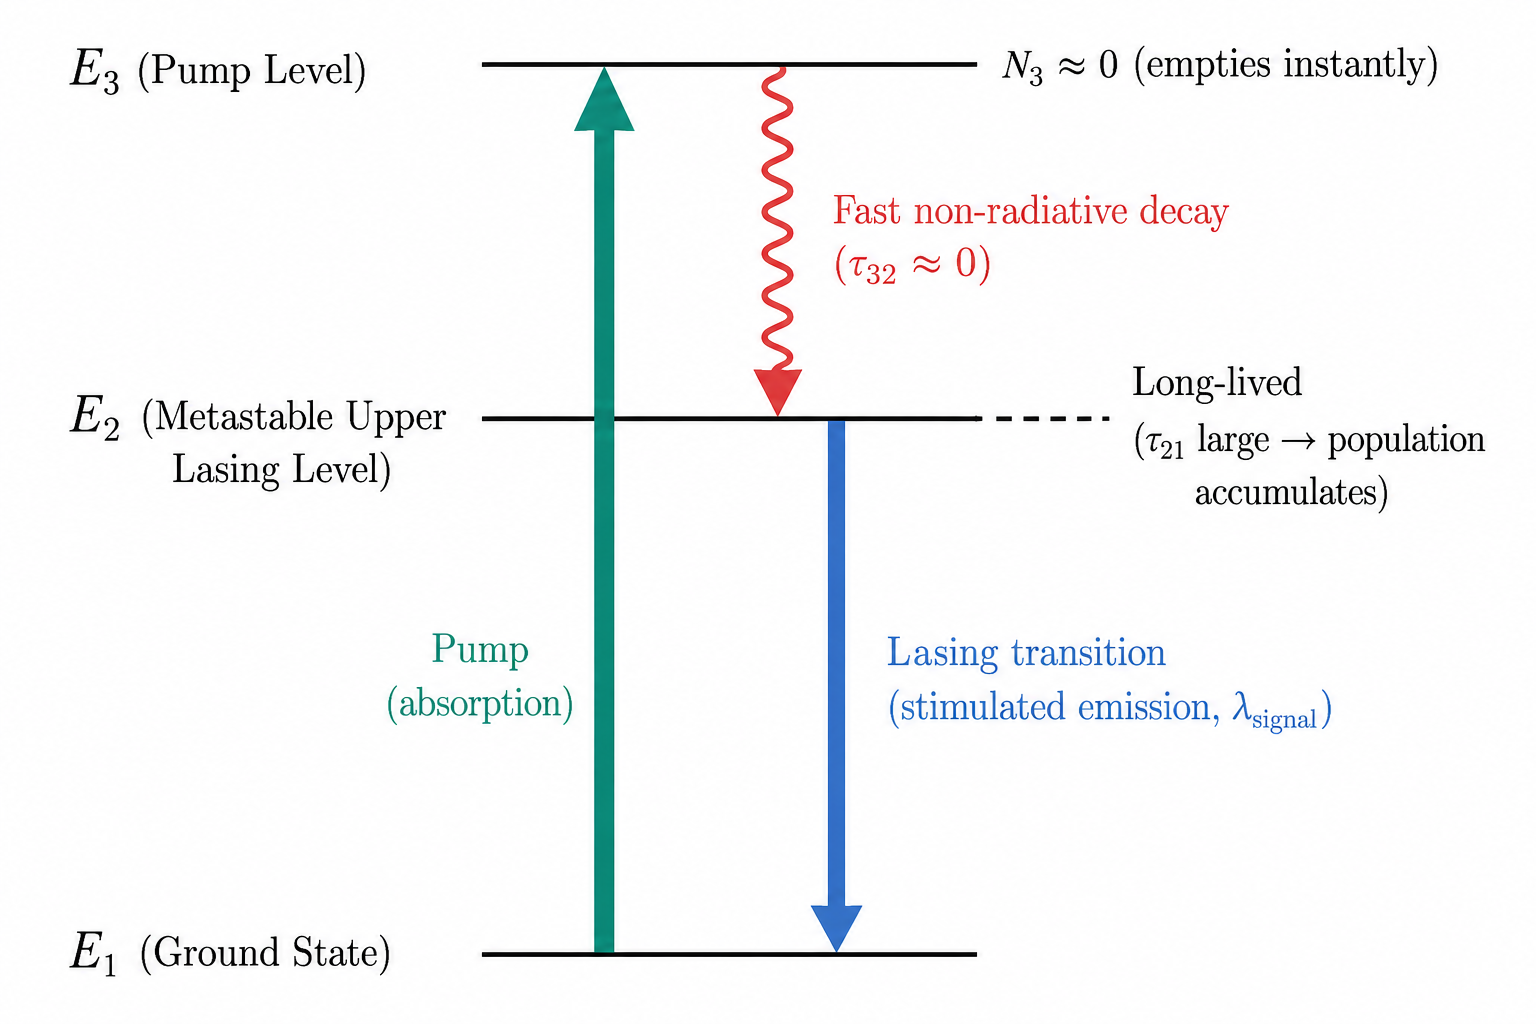
\includegraphics[width=0.6\textwidth]{Figures/Chapter 3/three_level_pumping_architecture.jpg}
    \caption{System Architecture: Physical realization of a 3-level optical pumping scheme, showcasing the rapid non-radiative decay $\tau_{32}$ creating the population inversion bottleneck at $E_2$.}
\end{figure}

\subsection{Case 1: Constant Pump Rate, No Signal (\texorpdfstring{$\Phi = 0$}{Phi=0})}

We first ask: what population inversion can the pump establish \emph{before} any signal is present? To find out, we assume no external signal ($\Phi = 0$) and a constant generic pump pulling atoms up at a steady rate $R$ (units: atoms~m$^{-3}$~s$^{-1}$). Let us explicitly map out the processes governing the populations of the two upper levels, $N_3$ and $N_2$.

For the pump level $E_3$, there are two governing processes:
\begin{enumerate}
    \item \textbf{Pump Arrival:} Atoms are forced into $E_3$ from the ground state at a rate $+R$.
    \item \textbf{Thermal Cascade (Decay):} Atoms spontaneously drop from $E_3$ down to $E_2$ via non-radiative decay at a rate $-\frac{N_3}{\tau_{32}}$.
\end{enumerate}

Combining these, the differential rate equation for $N_3$ is:
\begin{equation}
    \frac{dN_3}{dt} = \underbrace{R}_{\text{Pump Up}} - \underbrace{\frac{N_3}{\tau_{32}}}_{\text{Decay to } E_2} \tag{I}
\end{equation}

For the metastable upper lasing level $E_2$, there are also two governing processes:
\begin{enumerate}
    \item \textbf{Cascade Arrival:} The exact same atoms decaying down from $E_3$ enter $E_2$ at a rate $+\frac{N_3}{\tau_{32}}$.
    \item \textbf{Spontaneous Emission (Decay):} Atoms slowly leak out of $E_2$ back to the ground state $E_1$ at a rate $-\frac{N_2}{\tau_{21}}$.
\end{enumerate}

The differential rate equation for $N_2$ is therefore:
\begin{equation}
    \frac{dN_2}{dt} = \underbrace{\frac{N_3}{\tau_{32}}}_{\text{Arrival from } E_3} - \underbrace{\frac{N_2}{\tau_{21}}}_{\text{Spont. Decay to } E_1} \tag{II}
\end{equation}

The equation for the ground state $N_1$ is mathematically redundant. Because the total number of atoms in the system is strictly conserved ($N_1 + N_2 + N_3 = N_a$), following any two populations automatically dictates the third. We therefore only need to solve \textup{(I)} and \textup{(II)}.

\subsubsection*{Steady-State Analysis}

To determine the final populations achievable by this pump, we let the system settle into steady state where the populations no longer change in time. We set the derivatives to zero.

Starting with the pump level $E_3$ by setting $dN_3/dt = 0$ in equation \textup{(I)}:
\begin{equation*}
    0 = R - \frac{N_3}{\tau_{32}} \quad \Longrightarrow \quad N_3 = R\,\tau_{32}
\end{equation*}
As we established in our design requirements, the $E_3 \to E_2$ decay is engineered to be instantaneous ($\tau_{32} \to 0$). Therefore:
\begin{equation*}
    N_3 \approx 0
\end{equation*}
This formally confirms that atoms never pile up in the uppermost level; they fall to the metastable shelf instantly.

Next, we evaluate the metastable shelf $E_2$ by setting $dN_2/dt = 0$ in equation \textup{(II)}:
\begin{equation*}
    0 = \frac{N_3}{\tau_{32}} - \frac{N_2}{\tau_{21}}
\end{equation*}
Substituting the steady-state relationship $N_3 = R\,\tau_{32}$ into equation \textup{(II)}:
\begin{equation*}
    0 = \frac{R\,\tau_{32}}{\tau_{32}} - \frac{N_2}{\tau_{21}} \quad \Longrightarrow \quad 0 = R - \frac{N_2}{\tau_{21}} \quad \Longrightarrow \quad N_2 = R\,\tau_{21}
\end{equation*}

With $N_2$ found and $N_3 = 0$, we find the ground state population $N_1$ using our strict atom conservation law:
\begin{equation*}
    N_1 = N_a - N_2 = N_a - R\,\tau_{21}
\end{equation*}

Finally, we calculate the general \textbf{population inversion} parameter $N \equiv N_2 - N_1$:
\begin{equation*}
    N = R\,\tau_{21} - (N_a - R\,\tau_{21}) \quad \Longrightarrow \quad N = 2R\,\tau_{21} - N_a
\end{equation*}

However, because this specific derivation assumes there is absolutely no external signal saturating the system ($\Phi = 0$), this is purely the baseline \textbf{small-signal population inversion}. We therefore formally lock this maximum undisturbed value in as $N_0$:
\begin{keyresult}
\begin{equation}
    N_0 = 2R\tau_{21} - N_a
\end{equation}
\end{keyresult}

Because this value represents the undisturbed maximum inversion before any signal begins to deplete it ($\Phi = 0$), it directly establishes the \textbf{small-signal gain coefficient} ($\gamma_0$) of the amplifier:
\begin{keyresult}
\begin{equation}
    \gamma_0 = \sigma N_0 = \sigma(2R\tau_{21} - N_a)
\end{equation}
\end{keyresult}

\subsubsection*{Threshold Pump Rate}

For optical amplification to be physically possible, the inversion must be strictly positive ($N_0 > 0$, and therefore $\gamma_0 > 0$). Enforcing this condition:
\begin{equation*}
    2R\tau_{21} - N_a > 0 \quad \Longrightarrow \quad 2R\tau_{21} > N_a
\end{equation*}

\begin{keyresult}
\begin{equation}
    R > R_\text{th} \equiv \frac{N_a}{2\tau_{21}}
\end{equation}
\end{keyresult}

This is the \textbf{threshold pump rate}. Physically, the pump excites atoms from the ground state $E_1$ into $E_3$, which instantly cascade down to fill the metastable $E_2$ shelf. Because the lower lasing level is the ground state itself, achieving inversion ($N_2 > N_1$) inherently requires relocating more than half the total atomic population ($N_a/2$) into $E_2$ just to break even.

\subsection{Case 2: Constant Pump Rate, With Signal (\texorpdfstring{$\Phi \neq 0$}{Phi not=0})}

Now we introduce the optical signal: $\Phi \neq 0$. The pump continues to run at a constant rate $R$, but the signal now actively drives stimulated transitions between $E_1$ and $E_2$. Let us explicitly map out the physical processes.

For the pump level $E_3$, the governing processes remain unchanged from before:
\begin{enumerate}
    \item \textbf{Pump Arrival:} Atoms are forced into $E_3$ at a constant rate $+R$.
    \item \textbf{Thermal Cascade (Decay):} Atoms drop down to $E_2$ at a rate $-\frac{N_3}{\tau_{32}}$.
\end{enumerate}

The differential rate equation for $N_3$ is identical:
\begin{equation}
    \frac{dN_3}{dt} = \underbrace{R}_{\text{Pump Up}} - \underbrace{\frac{N_3}{\tau_{32}}}_{\text{Decay to } E_2} \tag{I}
\end{equation}

For the metastable upper lasing level $E_2$, we now have three governing processes:
\begin{enumerate}
    \item \textbf{Cascade Arrival:} Atoms entering from $E_3$ at a rate $+\frac{N_3}{\tau_{32}}$.
    \item \textbf{Spontaneous Emission (Decay):} Atoms spontaneously leaking down to $E_1$ at a rate $-\frac{N_2}{\tau_{21}}$.
    \item \textbf{Net Stimulated Transitions:} The signal actively forces atoms out of $E_2$ (stimulated emission) and atoms into $E_2$ (stimulated absorption). Because both processes are identically driven by the external field $\Phi$, they are grouped into a single net downward rate: $-\sigma\Phi(N_2 - N_1)$.
\end{enumerate}

The differential rate equation for $N_2$ expands to:
\begin{equation}
    \frac{dN_2}{dt} = \underbrace{\frac{N_3}{\tau_{32}}}_{\text{Arrival from } E_3} - \underbrace{\frac{N_2}{\tau_{21}}}_{\text{Spont. Decay}} - \underbrace{\sigma\Phi(N_2 - N_1)}_{\text{Net Stimulated Exit}} \tag{II}
\end{equation}

As before, the equation for $N_1$ is redundant thanks to the conservation constraint ($N_1 + N_2 + N_3 = N_a$). We proceed with \textup{(I)} and \textup{(II)}.

\subsubsection*{Steady-State Analysis}

Setting the derivatives to zero for steady state, the pump level again yields $N_3 = R\,\tau_{32}$. Substituting this relationship into equation \textup{(II)}:
\begin{equation*}
    0 = \frac{R\,\tau_{32}}{\tau_{32}} - \frac{N_2}{\tau_{21}} - \sigma\Phi(N_2 - N_1) \quad \Longrightarrow \quad 0 = R - \frac{N_2}{\tau_{21}} - \sigma\Phi(N_2 - N_1)
\end{equation*}

To simplify the stimulated term, we use our fundamental definition $N \equiv N_2 - N_1$:
\begin{equation*}
    R = \frac{N_2}{\tau_{21}} + \sigma\Phi\,N
\end{equation*}

Because our ultimate engineering goal is to derive a steady-state equation purely for the macroscopic population inversion $N$ (since $N$ dictates the optical gain $\gamma = \sigma N$), we must eliminate the standalone microscopic variable $N_2$. From the conservation law (with $N_3 = 0$), we have $N_1 = N_a - N_2$. Substituting this into $N$ and solving for $N_2$:
\begin{equation*}
    N = N_2 - (N_a - N_2) = 2N_2 - N_a \quad \Longrightarrow \quad N_2 = \frac{N + N_a}{2}
\end{equation*}

Substitute this into our steady-state balance, isolate the $N$ terms, and factor:
\begin{equation*}
    R = \frac{N + N_a}{2\tau_{21}} + \sigma\Phi\,N \quad \Longrightarrow \quad R = \frac{N_a}{2\tau_{21}} + \frac{N}{2\tau_{21}} + \sigma\Phi\,N \quad \Longrightarrow \quad R - \frac{N_a}{2\tau_{21}} = N\!\left(\frac{1}{2\tau_{21}} + \sigma\Phi\right)
\end{equation*}

Divide to explicitly solve for $N$, then multiply numerator and denominator by $2\tau_{21}$ to clear the complex fractions:
\begin{equation*}
    N = \frac{R - \dfrac{N_a}{2\tau_{21}}}{\dfrac{1}{2\tau_{21}} + \sigma\Phi} \quad \Longrightarrow \quad N = \frac{2R\tau_{21} - N_a}{1 + 2\sigma\Phi\tau_{21}}
\end{equation*}

We immediately recognise the numerator as $N_0 = 2R\tau_{21} - N_a$ --- exactly the \textbf{small-signal population inversion} we derived in Case 1. To express the denominator in the standard normalized form, we group the fundamental physical constants scaling the signal $\Phi$ and formally define them as the inverse of the \textbf{saturation photon flux density}:
\begin{equation*}
    \Phi_s \equiv \frac{1}{2\sigma\tau_{21}}
\end{equation*}

Substituting these definitions, we arrive precisely at the universal saturation model:
\begin{keyresult}
\begin{equation}
    N = \frac{N_0}{1 + \Phi/\Phi_s}
\end{equation}
\end{keyresult}

This mathematically proves that the introduction of an optical signal ($\Phi \neq 0$) strictly saturates the population inversion. By aggressively driving net stimulated emission, the signal actively depletes the metastable shelf, dynamically forcing the inversion down below its undisturbed ceiling ($N_0$). The corresponding saturated gain coefficient is found directly by multiplying both sides by $\sigma$:
\begin{keyresult}
\begin{equation*}
    \gamma = \sigma N = \frac{\sigma N_0}{1 + \Phi/\Phi_s} = \frac{\gamma_0}{1 + \Phi/\Phi_s}
\end{equation*}
\end{keyresult}

\begin{keyinsight}[The Physics of the Saturation Flux $\Phi_s$]
If an incoming signal ever grows intense enough to exactly reach the threshold $\Phi = \Phi_s$, the population inversion is mathematically crushed to exactly half of its unperturbed value ($N = N_0/2$). It is the absolute tipping point of saturation. Furthermore, the physics mapped inside the isolated constant ($\Phi_s \equiv \frac{1}{2\sigma\tau_{21}}$) are brilliant: materials with a large cross section $\sigma$ (highly susceptible to stimulation) or long spontaneous lifetime $\tau_{21}$ (atoms waiting a long time to interact) are inherently fragile. Their saturation threshold $\Phi_s$ drops drastically low, causing them to saturate much earlier.
\end{keyinsight}

\subsubsection*{Threshold Pump Rate}

For optical amplification to be physically possible, $N_0$ must be strictly positive ($N_0 > 0$, and therefore $\gamma_0 > 0$). Since $N_0 = 2R\tau_{21} - N_a$, enforcing this condition yields:
\begin{equation*}
    2R\tau_{21} - N_a > 0 \quad \Longrightarrow \quad R > \frac{N_a}{2\tau_{21}}
\end{equation*}
\begin{keyresult}
\begin{equation}
    R > R_\text{th} \equiv \frac{N_a}{2\tau_{21}}
\end{equation}
\end{keyresult}

This is the exact same threshold derived in Case 1 — and it must be. The threshold is purely a property of the pump establishing $N_0$, which in this model is still determined entirely by $R$. The signal $\Phi$ can only saturate an inversion that already exists; it cannot create one.

\subsection{Case 3: Optical Pump, With Signal (\texorpdfstring{$\Phi \neq 0$, $R = \sigma_p\Phi_p N_1$}{realistic pump model})}

In a real, physical optical pumping scheme, the pump rate is \emph{not} an abstract independent constant. A pump laser of photon flux density $\Phi_p$ relies on atomic absorption to do its work. Therefore, the rate at which it forces atoms out of $E_1$ depends directly on how many atoms are actually sitting in $E_1$ available to be absorbed:
\begin{equation*}
    R = \sigma_p\,\Phi_p\,N_1
\end{equation*}
where $\sigma_p$ is the absorption cross-section specifically for the $E_1 \to E_3$ pump transition.

This is the most physically realistic operational model of the three, and it is identically the one underpinning the \textbf{Erbium-Doped Fibre Amplifier (EDFA)} analysis later in this course. Let us explicitly map out the physical processes governing all three levels.

For the pump level $E_3$, there are two governing processes:
\begin{enumerate}
    \item \textbf{Optical Pump Arrival:} The pump laser actively absorbs atoms out of the ground state $E_1$ and forces them into $E_3$ at a field-driven rate $+\sigma_p\Phi_p N_1$. Crucially, this rate scales with however many atoms are currently available in $E_1$.
    \item \textbf{Thermal Cascade (Decay):} Atoms rapidly drop from $E_3$ down to the metastable $E_2$ shelf via non-radiative decay at a rate $-\frac{N_3}{\tau_{32}}$.
\end{enumerate}

The differential rate equation for $N_3$ is therefore:
\begin{equation}
    \frac{dN_3}{dt} = \underbrace{\sigma_p\Phi_p N_1}_{\text{Optical Pump Up}} - \underbrace{\frac{N_3}{\tau_{32}}}_{\text{Decay to } E_2} \tag{I}
\end{equation}

For the metastable upper lasing level $E_2$, there are three governing processes:
\begin{enumerate}
    \item \textbf{Cascade Arrival:} Atoms decaying out of $E_3$ enter $E_2$ at the same rate $+\frac{N_3}{\tau_{32}}$.
    \item \textbf{Spontaneous Emission (Decay):} Atoms slowly leak out of the metastable shelf back to $E_1$ at a rate $-\frac{N_2}{\tau_{21}}$.
    \item \textbf{Net Stimulated Transitions:} The signal actively forces atoms out of $E_2$ (stimulated emission) and atoms into $E_2$ (stimulated absorption). Because both processes are identically driven by the external field $\Phi$, they collapse into a single net downward rate: $-\sigma\Phi(N_2 - N_1)$.
\end{enumerate}

The differential rate equation for $N_2$ is therefore:
\begin{equation}
    \frac{dN_2}{dt} = \underbrace{\frac{N_3}{\tau_{32}}}_{\text{Arrival from } E_3} - \underbrace{\frac{N_2}{\tau_{21}}}_{\text{Spont. Decay}} - \underbrace{\sigma\Phi(N_2 - N_1)}_{\text{Net Stimulated Exit}} \tag{II}
\end{equation}

As before, the equation for $N_1$ is redundant thanks to the conservation constraint ($N_1 + N_2 + N_3 = N_a$). We proceed with \textup{(I)} and \textup{(II)}.

\subsubsection*{Steady-State Analysis}

Starting with the pump level $E_3$ by setting $dN_3/dt = 0$ in equation \textup{(I)}:
\begin{equation*}
    0 = \sigma_p\Phi_p N_1 - \frac{N_3}{\tau_{32}} \quad \Longrightarrow \quad N_3 = \sigma_p\Phi_p N_1 \tau_{32}
\end{equation*}

Next, we evaluate $E_2$ by setting $dN_2/dt = 0$ in equation \textup{(II)}, then substituting the steady-state relationship $N_3 = \sigma_p\Phi_p N_1\tau_{32}$ directly into its arrival term:
\begin{equation*}
    0 = \frac{\sigma_p\Phi_p N_1 \tau_{32}}{\tau_{32}} - \frac{N_2}{\tau_{21}} - \sigma\Phi(N_2 - N_1) \quad \Longrightarrow \quad 0 = \sigma_p\Phi_p N_1 - \frac{N_2}{\tau_{21}} - \sigma\Phi(N_2 - N_1)
\end{equation*}

Because our ultimate engineering goal is to derive a master equation purely for the macroscopic population inversion $N$, we must eliminate the standalone $N_1$ and $N_2$ variables. Using our conservation identities $N_2 = (N_a + N)/2$ and $N_1 = (N_a - N)/2$, we inject them straight into the balance equation:
\begin{equation*}
    \sigma_p\Phi_p\!\left(\frac{N_a - N}{2}\right) - \frac{(N_a + N)/2}{\tau_{21}} - \sigma\Phi\,N = 0
\end{equation*}

Multiply the entire equation by $2\tau_{21}$ to clear the nested fractions, then distribute all terms:
\begin{equation*}
    \sigma_p\Phi_p\tau_{21}(N_a - N) - (N_a + N) - 2\sigma\Phi\tau_{21}\,N = 0 \quad \Longrightarrow \quad \sigma_p\Phi_p\tau_{21}N_a - \sigma_p\Phi_p\tau_{21}N - N_a - N - 2\sigma\Phi\tau_{21}N = 0
\end{equation*}

Isolate all terms containing $N$ on the right and factor algebraically:
\begin{equation*}
    N + \sigma_p\Phi_p\tau_{21}N + 2\sigma\Phi\tau_{21}N = N_a\sigma_p\Phi_p\tau_{21} - N_a \quad \Longrightarrow \quad N\!\left(1 + \sigma_p\Phi_p\tau_{21} + 2\sigma\Phi\tau_{21}\right) = N_a(\sigma_p\Phi_p\tau_{21} - 1)
\end{equation*}

Divide to explicitly solve for the macroscopic population inversion $N$:
\begin{equation*}
    N = N_a\,\frac{\sigma_p\Phi_p\tau_{21} - 1}{1 + \sigma_p\Phi_p\tau_{21} + 2\sigma\Phi\tau_{21}}
\end{equation*}

We calculate the general \textbf{population inversion} $N$ first, then evaluate its undisturbed ceiling by assuming there is no signal present ($\Phi = 0$). This establishes the baseline \textbf{small-signal population inversion} $N_0$:
\begin{keyresult}
\begin{equation}
    N_0 = N_a\,\frac{\sigma_p\Phi_p\tau_{21} - 1}{1 + \sigma_p\Phi_p\tau_{21}}
\end{equation}
\end{keyresult}

Because this value represents the undisturbed maximum inversion before any signal begins to deplete it, it directly establishes the \textbf{small-signal gain coefficient} ($\gamma_0$) of the amplifier:
\begin{keyresult}
\begin{equation}
    \gamma_0 = \sigma N_0 = \sigma N_a\,\frac{\sigma_p\Phi_p\tau_{21} - 1}{1 + \sigma_p\Phi_p\tau_{21}}
\end{equation}
\end{keyresult}

Now, returning to our general $N$ expression (with the signal $\Phi$ present), we express the denominator in the standard normalized form by factoring out the leading $(1 + \sigma_p\Phi_p\tau_{21})$ term:
\begin{equation*}
    N = N_a\,\frac{\sigma_p\Phi_p\tau_{21} - 1}{1 + \sigma_p\Phi_p\tau_{21} + 2\sigma\Phi\tau_{21}} \quad \Longrightarrow \quad N = N_a\,\frac{\sigma_p\Phi_p\tau_{21} - 1}{(1 + \sigma_p\Phi_p\tau_{21})\!\left(1 + \dfrac{2\sigma\Phi\tau_{21}}{1 + \sigma_p\Phi_p\tau_{21}}\right)}
\end{equation*}

The numerator and the extracted $(1 + \sigma_p\Phi_p\tau_{21})$ from the denominator now combine exactly into $N_0$. The remaining constants multiplying $\Phi$ in the denominator formally define the inverse of the \textbf{saturation photon flux density}:
\begin{equation*}
    \Phi_s \equiv \frac{1 + \sigma_p\Phi_p\tau_{21}}{2\sigma\tau_{21}}
\end{equation*}

Substituting these definitions, the fully realistic optical pumping model collapses cleanly into the same universal saturation form:
\begin{keyresult}
\begin{equation}
    N = \frac{N_0}{1 + \Phi/\Phi_s} \quad \Longrightarrow \quad \gamma = \frac{\gamma_0}{1 + \Phi/\Phi_s}
\end{equation}
\end{keyresult}

\subsubsection*{Threshold Condition}

For optical amplification to be physically possible, the inversion must be strictly positive ($N_0 > 0$, and therefore $\gamma_0 > 0$). Enforcing this condition dictates that the numerator of $N_0$ must cross zero:
\begin{equation*}
    \sigma_p\Phi_p\tau_{21} - 1 > 0 \quad \Longrightarrow \quad \Phi_p > \frac{1}{\sigma_p\tau_{21}}
\end{equation*}
\begin{keyresult}
\begin{equation}
    \Phi_p > \Phi_{p,\text{th}} \equiv \frac{1}{\sigma_p\tau_{21}}
\end{equation}
\end{keyresult}

This is the \textbf{threshold pump photon flux}. Physically, the pump laser must deliver photons fast enough to evacuate atoms out of $E_1$ into $E_3$ at a greater rate than they spontaneously cycle back. Without crossing this precise photon delivery rate, net inversion can never accumulate.

All three physical models successfully converge on the exact same universal saturation form $N = N_0/(1 + \Phi/\Phi_s)$. The formulas for $N_0$ and $\Phi_s$ simply adapt to accommodate the mathematical realism of the pumping mechanism.

\subsection{Comparison of the Three Pumping Models}

The three cases we have analysed represent increasing levels of physical realism — from an idealized constant pump with no signal, to a constant pump driving stimulated emission, to a fully self-consistent optical pump model. The table below collects the key steady-state parameters for direct comparison across all three regimes.

\begin{table}[H]
\centering
\begin{tabular}{@{} >{\raggedright\arraybackslash}p{0.18\textwidth} >{\centering\arraybackslash}p{0.36\textwidth} >{\centering\arraybackslash}p{0.38\textwidth} @{}}
\toprule
\textbf{Parameter} & \textbf{Cases 1 \& 2} (Constant $R$) & \textbf{Case 3} (Optical Pump $\sigma_p\Phi_p N_1$) \\
\midrule
$N_0$ & $2R\tau_{21} - N_a$ & $N_a\,\dfrac{\sigma_p\Phi_p\tau_{21} - 1}{1 + \sigma_p\Phi_p\tau_{21}}$ \\[2ex]
$\gamma_0$ & $\sigma(2R\tau_{21} - N_a)$ & $\sigma N_a\,\dfrac{\sigma_p\Phi_p\tau_{21} - 1}{1 + \sigma_p\Phi_p\tau_{21}}$ \\[2ex]
$\Phi_s$ & $\dfrac{1}{2\sigma\tau_{21}}$ & $\dfrac{1 + \sigma_p\Phi_p\tau_{21}}{2\sigma\tau_{21}}$ \\[2ex]
Threshold & $R > \dfrac{N_a}{2\tau_{21}}$ & $\Phi_p > \dfrac{1}{\sigma_p\tau_{21}}$ \\
\bottomrule
\end{tabular}
\caption{Summary of key steady-state parameters across the three pumping models.}
\end{table}

Several important physical observations follow directly from this comparison:

\begin{enumerate}
    \item \textbf{$N_0$ is unbounded in Cases 1 \& 2, but bounded in Case 3.} With a constant pump $R$, the small-signal inversion $N_0 = 2R\tau_{21} - N_a$ grows without limit as $R$ increases. In Case 3, however, $N_0$ asymptotes strictly to $+N_a$ as $\Phi_p \to \infty$ — because you can never invert more atoms than you have in the system.

    \item \textbf{$\Phi_s$ is a fixed material constant in Cases 1 \& 2, but pump-dependent in Case 3.} In the constant-$R$ model, $\Phi_s = 1/(2\sigma\tau_{21})$ depends only on intrinsic material properties; every amplifier operating with the same gain medium saturates at the same signal level. In Case 3, $\Phi_s$ increases with pump strength $\Phi_p$ — a stronger pump actively fights back against signal-driven depletion of $E_2$, making the amplifier harder to saturate. This is a direct consequence of the self-consistent feedback loop: as stimulated emission drains $E_1 \to E_2$ back into $E_1$, a stronger pump immediately re-evacuates those atoms.

    \item \textbf{Cases 1 \& 2 share the same threshold, Case 3 introduces a new one.} Both constant-pump cases require $R > N_a/2\tau_{21}$ to achieve inversion. Case 3 translates this into a photon flux threshold $\Phi_p > 1/(\sigma_p\tau_{21})$, which states that the pump must deliver photons fast enough to keep the upward pumping rate faster than the spontaneous relaxation rate.

    \item \textbf{The universal saturation form is exact in all three cases.} Despite the different levels of physical realism, all three models collapse precisely to $N = N_0/(1+\Phi/\Phi_s)$. This is not an approximation — it is an exact consequence of the three-level steady-state algebra in each regime.
\end{enumerate}

% =============================================================
\section{Parameters of an Optical Amplifier}
% =============================================================

Now that we know how to create population inversion and how the signal grows or saturates, we can characterise our \textbf{optical amplifier} properly. Any amplifier — optical or electronic — is described by three fundamental parameters: \textbf{gain} $G$, \textbf{bandwidth} $\Delta\nu$, and \textbf{noise performance}. Let's find each one.

% ------- GAIN -------------------------------------------------
\subsection{Gain \texorpdfstring{$G$}{G}}

The gain of any amplifier is the ratio of output power to input power:
\begin{equation*}
  G = \frac{P_\text{out}}{P_\text{in}}
\end{equation*}

We must now find explicit expressions for $G$ in both operating regimes.

\subsubsection{Case 1: Small-Signal Gain $G_0$}

As we already know from the small-signal section, when $P_\text{in} \ll P_s$, the gain coefficient is constant: $\gamma = \gamma_0$. 

\begin{figure}[H]
    \centering
    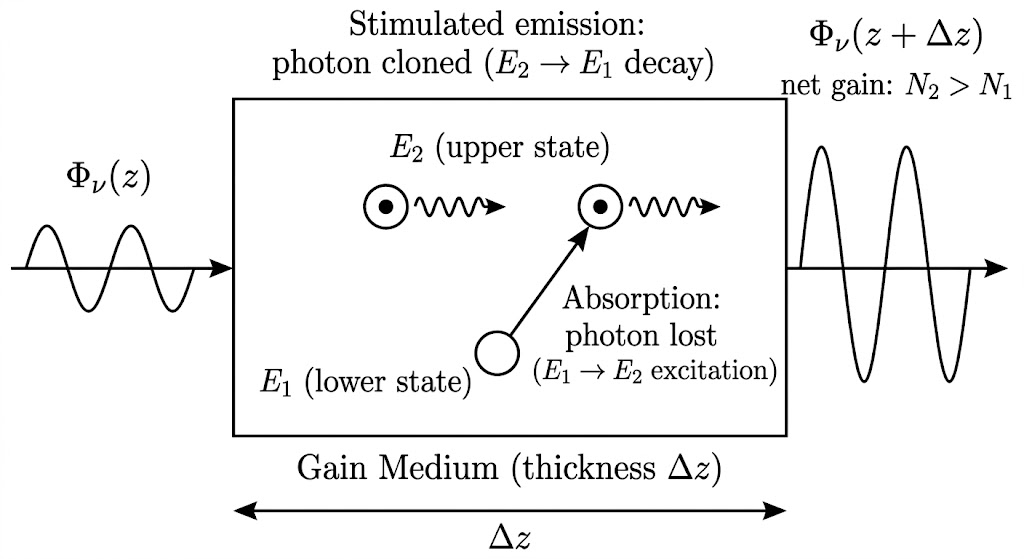
\includegraphics[width=0.6\textwidth]{Figures/Chapter 3/differential_gain_slab.jpg}
    \caption{Differential Gain Slab: Visualising the integration over a slice $dz$ of the active medium, where the power change $dP$ scales strictly with the local power $P$.}
\end{figure}

The propagation equation across this slice is:
\begin{equation*}
  \frac{dP}{dz} = \gamma_0\,P
\end{equation*}
Integrating from $z=0$ to $z=L$ (where $L$ is the physical length of the gain medium):
\begin{equation*}
  \int_{P_\text{in}}^{P_\text{out}} \frac{dP}{P} = \int_0^L \gamma_0\,dz
\end{equation*}
\begin{equation*}
  \left[\ln P\right]_{P_\text{in}}^{P_\text{out}} = \gamma_0\,L
\end{equation*}
\begin{equation*}
  \ln P_\text{out} - \ln P_\text{in} = \gamma_0\,L
\end{equation*}
Using the logarithm rule $\ln a - \ln b = \ln(a/b)$:
\begin{equation*}
  \ln\!\left(\frac{P_\text{out}}{P_\text{in}}\right) = \gamma_0\,L
\end{equation*}
Exponentiating both sides:
\begin{equation*}
  \frac{P_\text{out}}{P_\text{in}} = e^{\gamma_0 L}
\end{equation*}
Therefore the small-signal gain is:
\begin{keyresult}
\begin{equation}
  G_0 = e^{\gamma_0 L}
\end{equation}
\end{keyresult}
In decibels:
\begin{equation*}
  G_0\big|_\text{dB} = 10\log_{10}\!\left(e^{\gamma_0 L}\right) = 10\,\gamma_0 L\,\log_{10} e \approx 4.343\,\gamma_0 L \; \text{(dB)}
\end{equation*}

This is the \textbf{small-signal gain}: it depends only on the gain coefficient $\gamma_0$ and the amplifier length $L$. Since $\gamma_0 = \sigma N_0$, a longer amplifier or a more strongly inverted medium gives a higher small-signal gain.

Therefore, while still safely in the small-signal regime, the total gain holds its pure exponential form $G_0 = e^{\gamma_0 L}$. This value is perfectly determined by merely the per-unit-length gain coefficient and the physical length constraint of the active medium.

\subsubsection{Case 2: General (Saturated) Gain $G$}

When $P_\text{in}$ is comparable to $P_s$, the gain coefficient is no longer constant:
\begin{equation*}
  \frac{dP}{dz} = \gamma\,P = \frac{\gamma_0}{1+P/P_s}\,P
\end{equation*}
Rearranging to separate variables — multiply both sides by $(1+P/P_s)$ and divide by $P$:
\begin{equation*}
  \left(\frac{1}{P} + \frac{1}{P_s}\right) dP = \gamma_0\,dz
\end{equation*}
Integrating the left side from $P_\text{in}$ to $P_\text{out}$ and the right side from $0$ to $L$:
\begin{equation*}
  \int_{P_\text{in}}^{P_\text{out}} \frac{dP}{P} + \int_{P_\text{in}}^{P_\text{out}} \frac{dP}{P_s} = \int_0^L \gamma_0\,dz
\end{equation*}
Evaluating each integral:
\begin{equation*}
  \left[\ln P\right]_{P_\text{in}}^{P_\text{out}} + \frac{1}{P_s}\left[P\right]_{P_\text{in}}^{P_\text{out}} = \gamma_0\,L
\end{equation*}
\begin{equation*}
  \ln\!\left(\frac{P_\text{out}}{P_\text{in}}\right) + \frac{P_\text{out} - P_\text{in}}{P_s} = \gamma_0\,L
\end{equation*}
We now recognise that $\ln(P_\text{out}/P_\text{in}) = \ln G$ and $\gamma_0 L = \ln G_0$ (from the small-signal result). Substituting these:
\begin{equation*}
  \ln G + \frac{P_\text{in}}{P_s}\!\left(\frac{P_\text{out}}{P_\text{in}} - 1\right) = \ln G_0
\end{equation*}
\begin{equation*}
  \ln G + \frac{P_\text{in}}{P_s}(G - 1) = \ln G_0
\end{equation*}
Isolating $\ln G - \ln G_0$:
\begin{equation*}
  \ln G - \ln G_0 = -\frac{P_\text{in}}{P_s}(G-1)
\end{equation*}
Using the logarithm rule $\ln G - \ln G_0 = \ln(G/G_0)$:
\begin{equation*}
  \ln\!\left(\frac{G}{G_0}\right) = -\frac{P_\text{in}}{P_s}(G-1)
\end{equation*}
Exponentiating:
\begin{keyresult}
\begin{equation}
  G = G_0\,\exp\!\left(-\frac{P_\text{in}}{P_s}(G-1)\right)
\end{equation}
\end{keyresult}

This is the \textbf{saturated gain} expressed in terms of the small-signal gain $G_0 = e^{\gamma_0 L}$. Notice that when $P_\text{in} \ll P_s$, the exponential factor $\to 1$ and $G \to G_0$ — recovering our small-signal result as a special case. When $P_\text{in}$ is comparable to $P_s$, the negative exponent reduces $G$ below $G_0$: the gain compresses.

\begin{keyinsight}[Distinguishing $\gamma$ from $G$]
There is a very important distinction to keep in mind: $\gamma$ (or $\gamma_0$) is the \textbf{gain coefficient per unit length} (units m$^{-1}$), while $G$ is the \textbf{total power gain} of the amplifier (dimensionless). Some textbooks call both of them ``gain coefficient,'' which is confusing. Always check the context and the units. In our notation: $G_0 = e^{\gamma_0 L}$.
\end{keyinsight}

Tracing the full envelope, the gain of an optical amplifier effortlessly rides $G_0 = e^{\gamma_0 L}$ in the small-signal regime, but inevitably crashes back toward unity as the input power violently forces its way past the structural saturation power $P_s$.

\begin{figure}[H]
    \centering
    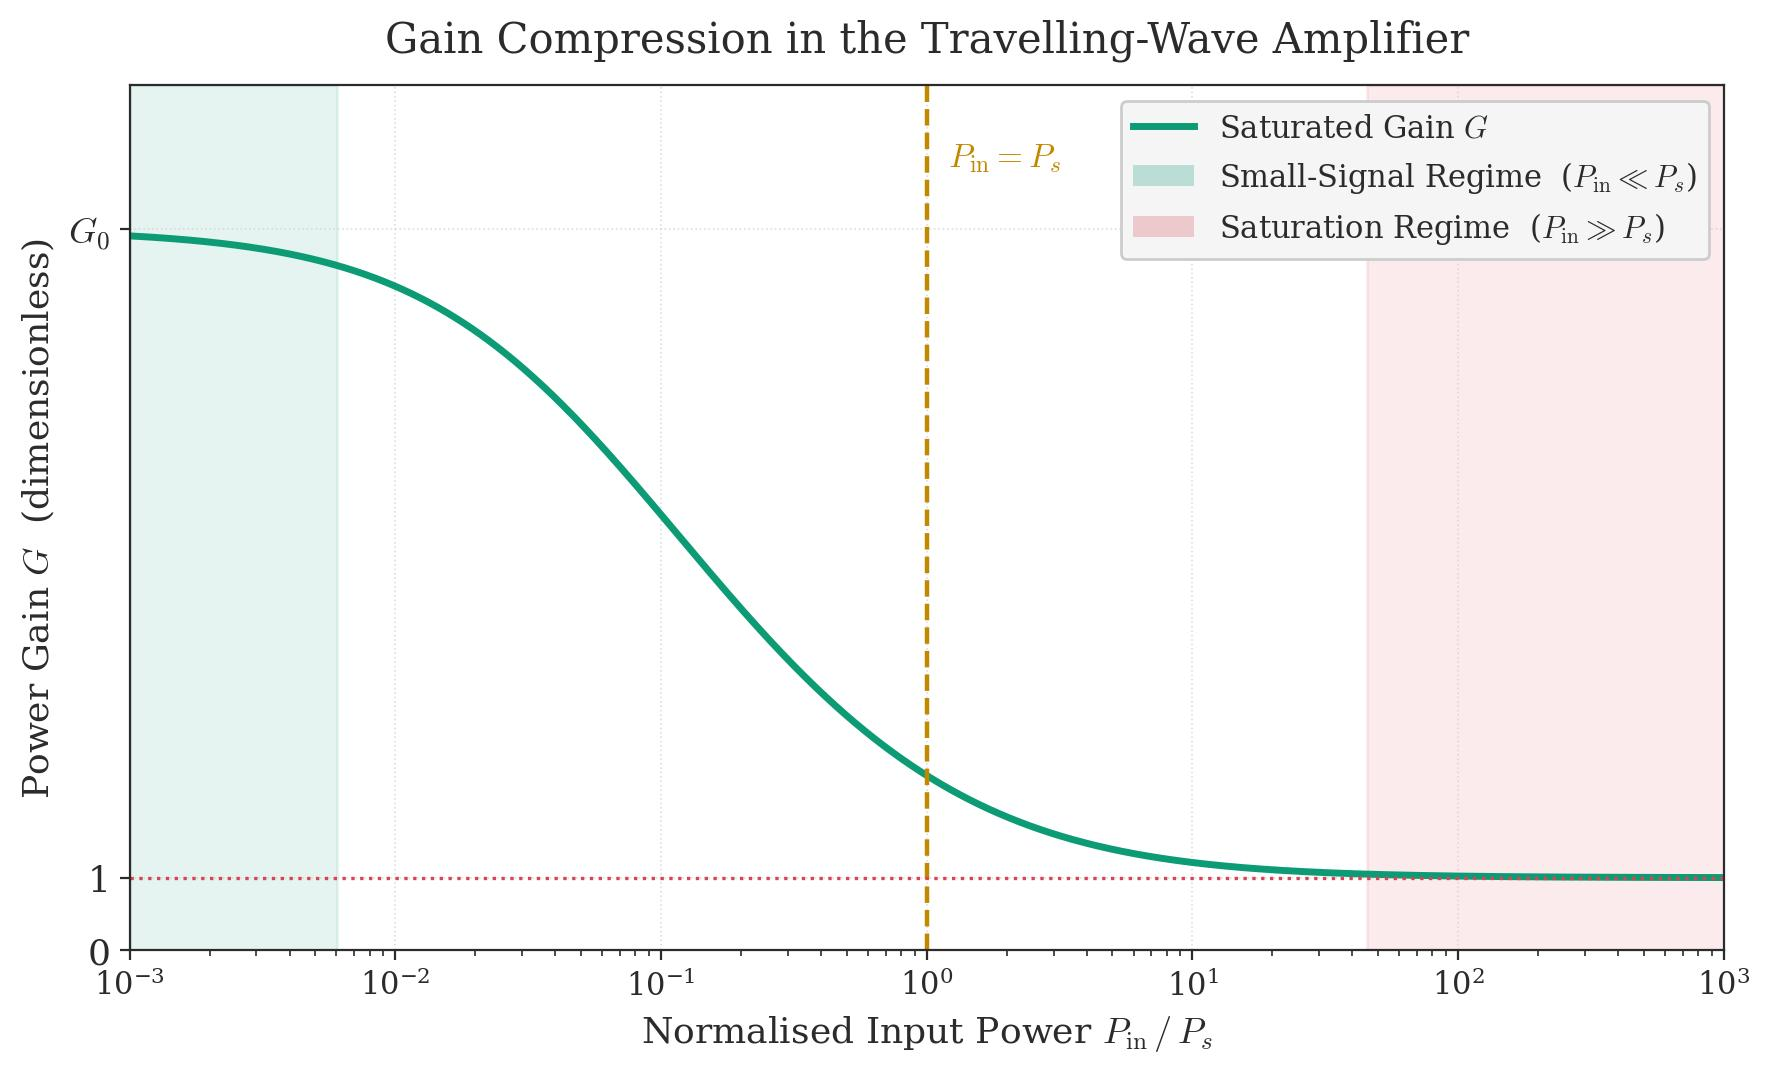
\includegraphics[width=0.7\textwidth]{Figures/Chapter 3/gain_compression.jpg}
    \caption{Gain Compression: The transition from the small-signal logarithmic gain $G_0$ region down to unity transmission as the input power heavily exceeds $P_s$.}
\end{figure}

% ------- BANDWIDTH --------------------------------------------
\subsection{Bandwidth \texorpdfstring{$\Delta\nu$}{Delta-nu}}

\begin{figure}[H]
    \centering
    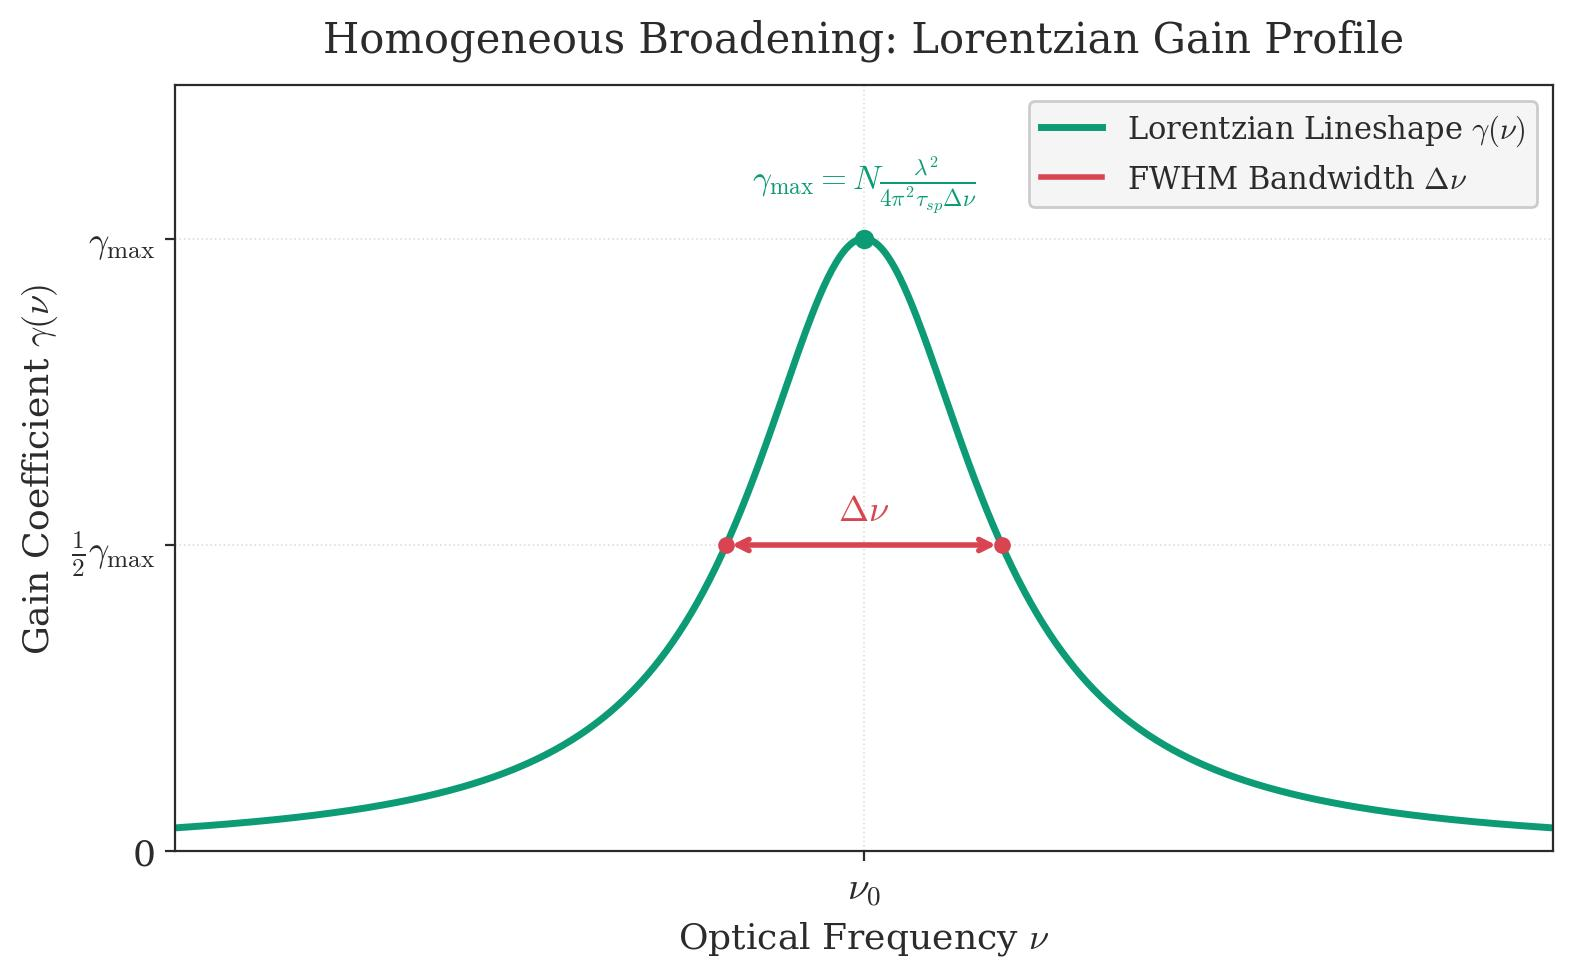
\includegraphics[width=0.7\textwidth]{Figures/Chapter 3/gain_coefficient_profile.jpg}
    \caption{Gain Coefficient Profile: A standard Lorentzian lineshape $\gamma_0(\nu)$ with a peak value $\gamma_{\text{max}}$ and an atomic linewidth FWHM $\Delta\nu$.}
\end{figure}

As we always do when characterising an amplifier, we find the bandwidth by plotting
the gain as a function of frequency and reading off the half-power width.  The key
subtlety here is that there are \emph{two} distinct quantities whose frequency
dependence we must track: the \textbf{gain coefficient} $\gamma_0(\nu)$ and the
\textbf{power gain} $G_0(\nu) = e^{\gamma_0(\nu)L}$.  They do not have the same
spectral shape, and confusing them is a common source of error.

\subsubsection*{Shape of \texorpdfstring{$\gamma_0(\nu)$}{gamma\_0(nu)}}

Since $\gamma_0 = \sigma(\nu)\,N_0$, and the cross-section
$\sigma(\nu)$ inherits its frequency dependence from the lineshape function
$g_{\nu_0}(\nu)$.  For homogeneous broadening the lineshape is a
\textbf{Lorentzian}, so:
\begin{keyresult}
\begin{equation}
    \gamma_0(\nu)
    = \frac{\gamma_{\max}}{1 + \left(\dfrac{2(\nu-\nu_0)}{\Delta\nu}\right)^2}
\end{equation}
\end{keyresult}
where $\gamma_{\max} \equiv \gamma_0(\nu_0)$ is the peak gain coefficient at the line
centre $\nu_0$, and $\Delta\nu$ is the FWHM of the Lorentzian — this is the
\textbf{atomic linewidth}.  For inhomogeneous (Doppler) broadening the lineshape is a
\textbf{Gaussian}:
\begin{equation*}
    \gamma_0(\nu)
    = \gamma_{\max}\,\exp\!\left(-\frac{(\nu-\nu_0)^2}{2\sigma_D^2}\right),
\end{equation*}
where $\sigma_D$ is the Doppler width parameter and the FWHM is
$\Delta\nu_D = 2\sqrt{2\ln 2}\,\sigma_D \approx 2.35\,\sigma_D$.

\subsubsection*{Shape of \texorpdfstring{$G_0(\nu)$}{G\_0(nu)}: Neither Lorentzian Nor Gaussian}

Now here is the important point: the small-signal power gain is
\begin{equation*}
    G_0(\nu) = e^{\gamma_0(\nu)\,L}.
\end{equation*}
Because the exponential function is nonlinear, $G_0(\nu)$ is \emph{not} the
same shape as $\gamma_0(\nu)$.  If $\gamma_0(\nu)$ is Lorentzian,
$e^{\gamma_0(\nu)L}$ is not Lorentzian.  If $\gamma_0(\nu)$ is Gaussian,
$e^{\gamma_0(\nu)L}$ is not Gaussian either.

This has a very important practical consequence:
the \textbf{bandwidth of $G_0$} (call it $\Delta\nu_{G_0}$) is always
\emph{narrower} than the atomic linewidth $\Delta\nu$ — a phenomenon called
\textbf{bandwidth narrowing} — whenever $G_0$ is large enough.  Let us now
derive the formula for $\Delta\nu_{G_0}$ precisely.

\subsubsection*{Deriving \texorpdfstring{$\Delta\nu_{G_0}$}{Delta-nu\_G0} for a Lorentzian Gain Profile}

We start with the peak gain:
\begin{equation}
    G_{0,\max} = e^{\gamma_{\max} L}. \tag{I} 
\end{equation}
By definition, the FWHM bandwidth $\Delta\nu_{G_0}$ of $G_0(\nu)$ is the
frequency separation at which $G_0$ falls to half its peak value.  Setting
$G_0(\nu_0 \pm \Delta\nu_{G_0}/2) = G_{0,\max}/2$:
\begin{equation}
    e^{\gamma_0(\nu_0 + \Delta\nu_{G_0}/2)\,L} = \frac{G_{0,\max}}{2}. \tag{II} 
\end{equation}
Taking the natural logarithm of both sides of \textup{(II)}:
\begin{equation*}
    \gamma_0\!\left(\nu_0 + \frac{\Delta\nu_{G_0}}{2}\right)\cdot L
    = \ln\!\left(\frac{G_{0,\max}}{2}\right).
\end{equation*}
Substituting the Lorentzian gain coefficient $\gamma_0(\nu) = \gamma_{\max}/\bigl[1+(2(\nu-\nu_0)/\Delta\nu)^2\bigr]$ with $\nu - \nu_0 = \Delta\nu_{G_0}/2$ into the left-hand side:
\begin{equation*}
    \frac{\gamma_{\max} L}{1 + \left(\dfrac{\Delta\nu_{G_0}}{\Delta\nu}\right)^2}
    = \ln\!\left(\frac{G_{0,\max}}{2}\right).
\end{equation*}
Substituting $\gamma_{\max}L = \ln(G_{0,\max})$ from \textup{(I)} into the left-hand side:
\begin{equation*}
    \frac{\ln(G_{0,\max})}{1 + \left(\dfrac{\Delta\nu_{G_0}}{\Delta\nu}\right)^2}
    = \ln\!\left(\frac{G_{0,\max}}{2}\right).
\end{equation*}
Dividing both sides by $\ln(G_{0,\max}/2)$:
\begin{equation*}
    \frac{\ln(G_{0,\max})}{\ln(G_{0,\max}/2)}
    = 1 + \left(\frac{\Delta\nu_{G_0}}{\Delta\nu}\right)^2.
\end{equation*}
Isolating the ratio $\Delta\nu_{G_0}/\Delta\nu$:
\begin{equation*}
    \left(\frac{\Delta\nu_{G_0}}{\Delta\nu}\right)^2
    = \frac{\ln(G_{0,\max})}{\ln(G_{0,\max}/2)} - 1.
\end{equation*}
Taking the square root (taking the positive root since both bandwidths are positive):
\begin{keyresult}
\begin{equation}
    \Delta\nu_{G_0}
    = \Delta\nu\,\sqrt{\frac{\ln(G_{0,\max})}{\ln(G_{0,\max}/2)} - 1}
\end{equation}
\end{keyresult}

where:
\begin{itemize}
    \item $\Delta\nu_{G_0}$: FWHM bandwidth of the amplifier power gain $G_0(\nu)$
    \item $\Delta\nu$: FWHM of the underlying atomic lineshape (bandwidth of $\gamma_0(\nu)$)
    \item $G_{0,\max} = e^{\gamma_{\max}L}$: peak small-signal gain, as defined in \textup{(I)} above
\end{itemize}

\subsubsection*{The Bandwidth-Narrowing Condition}

Now let us ask: is $\Delta\nu_{G_0}$ always less than $\Delta\nu$?  We need to check
when $\Delta\nu_{G_0} < \Delta\nu$, i.e. when the square root factor is less than 1:
\begin{equation*}
    \sqrt{\frac{\ln G_{0,\max}}{\ln(G_{0,\max}/2)} - 1} < 1
    \;\Longrightarrow\;
    \frac{\ln G_{0,\max}}{\ln(G_{0,\max}/2)} - 1 < 1
    \;\Longrightarrow\;
    \frac{\ln G_{0,\max}}{\ln(G_{0,\max}/2)} < 2.
\end{equation*}
Cross-multiplying by $\ln(G_{0,\max}/2) > 0$:
\begin{equation*}
    \ln G_{0,\max} < 2\ln(G_{0,\max}/2) = \ln(G_{0,\max}/2)^2 = \ln(G_{0,\max}^2/4).
\end{equation*}
Exponentiating:
\begin{equation*}
    G_{0,\max} < \frac{G_{0,\max}^2}{4}
    \;\Longrightarrow\;
    4 < G_{0,\max}.
\end{equation*}
So the bandwidth-narrowing condition is simply:
\begin{keyresult}
\begin{equation}
    G_{0,\max} > 4 \;\Longrightarrow\; \Delta\nu_{G_0} < \Delta\nu \quad
    \text{(bandwidth narrowing)}
\end{equation}
\end{keyresult}

This is the practical case for any useful amplifier.  If $G_{0,\max} \leq 4$, then
$\Delta\nu_{G_0} \geq \Delta\nu$ (the gain bandwidth equals or slightly exceeds the
atomic linewidth — not a useful amplifier regime).

The physical picture makes this intuitive: at the edges of the gain profile,
$\gamma_0(\nu)$ is small, so $G_0(\nu) = e^{\gamma_0(\nu)L}$ is barely above unity.
At the centre, $G_0 = e^{\gamma_{\max}L}$ is large.  The exponential
strongly amplifies the contrast between centre and edges, making the gain
profile sharper than the gain coefficient profile.  The higher $G_{0,\max}$ is,
the more pronounced this sharpening effect becomes.

Note also that at $\nu_0 \pm \Delta\nu/2$ (the atomic FWHM points), the gain
coefficient is $\gamma_{\max}/2$, so the gain there is:
\begin{equation*}
    G_0\!\left(\nu_0 \pm \frac{\Delta\nu}{2}\right)
    = e^{(\gamma_{\max}/2)L}
    = e^{\frac{1}{2}\gamma_{\max}L}
    = \sqrt{G_{0,\max}}.
\end{equation*}
Notice that at the atomic FWHM points, the amplifier gain is $\sqrt{G_{0,\max}}$, not
$G_{0,\max}/2$.  The amplifier's half-power point occurs at a \emph{closer} frequency
to $\nu_0$ than the atomic half-power point — hence the narrower bandwidth.

\begin{figure}[H]
    \centering
    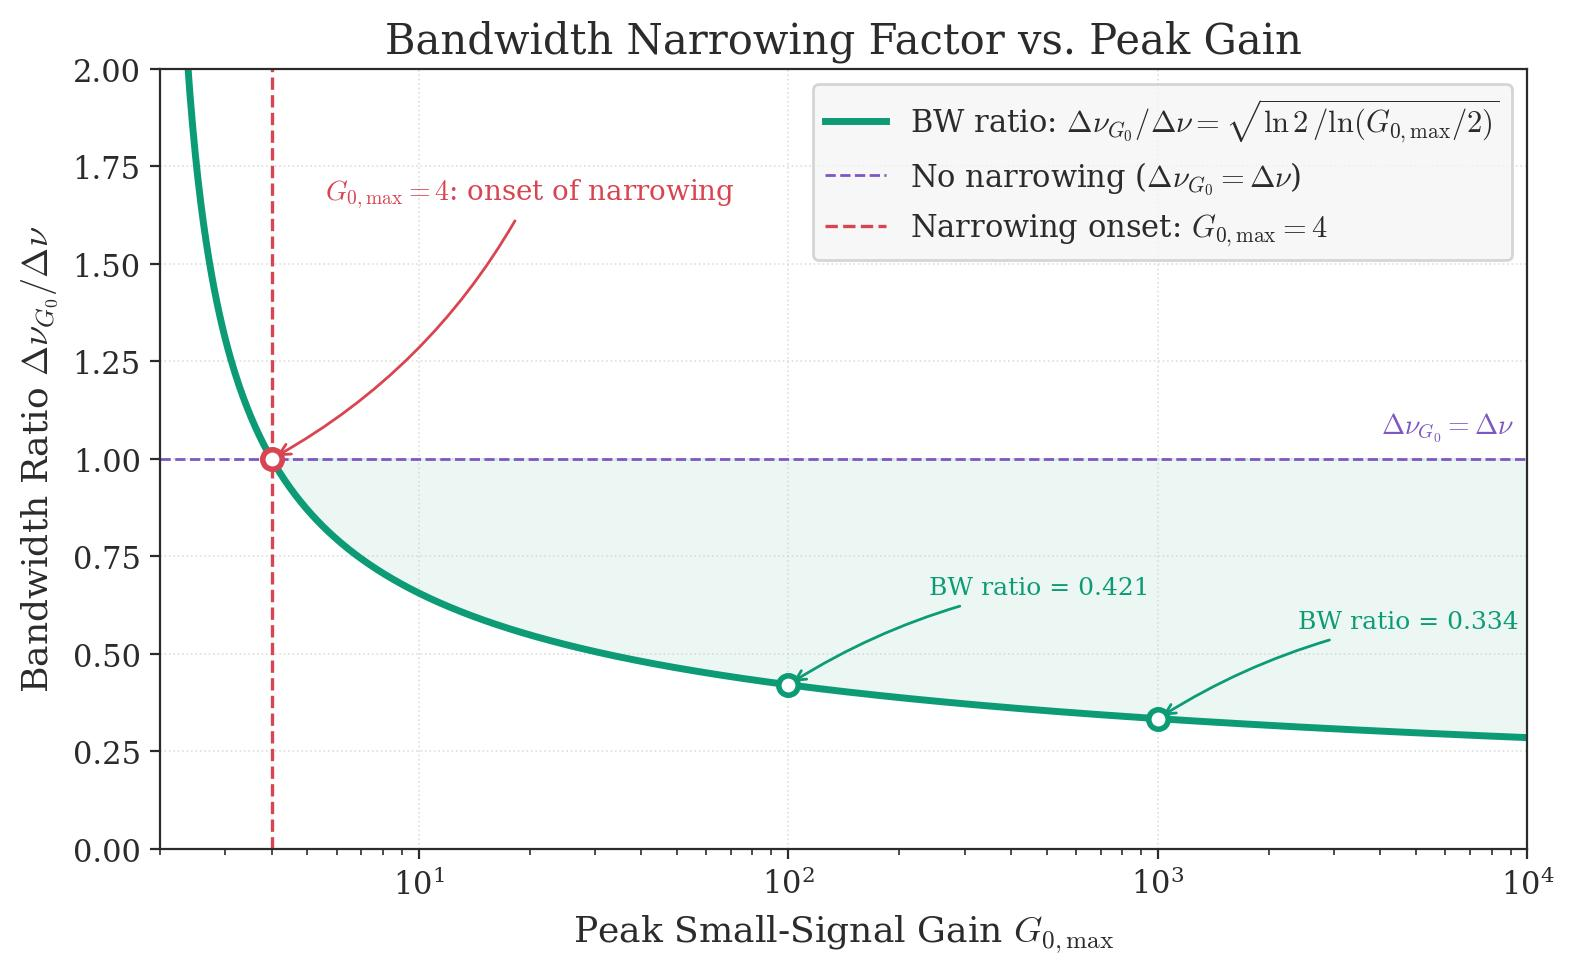
\includegraphics[width=0.7\textwidth]{Figures/Chapter 3/bandwidth_narrowing_exponential.jpg}
    \caption{Bandwidth Narrowing: Graphical proof that the $e^x$ exponential function sharply squashes the spectral width of $G_0(\nu)$ relative to the underlying Lorentzian $\gamma_0(\nu)$ profile.}
\end{figure}

The compounding math reveals a hidden cost: the amplifier's exponential power gain $G_0(\nu) = e^{\gamma_0(\nu)L}$ is structurally neither Lorentzian nor Gaussian, even when the underlying $\gamma_0(\nu)$ is remarkably clean. Its FWHM will aggressively sharpen, becoming strictly narrower than the intrinsic atomic linewidth anytime $G_{0,\max} > 4$, given explicitly by the ratio $\Delta\nu_{G_0}/\Delta\nu = \sqrt{\ln(G_{0,\max})/\ln(G_{0,\max}/2)-1}$ derived above. The harder we push the peak gain, the more severely we slice the available bandwidth.

\begin{figure}[H]
    \centering
    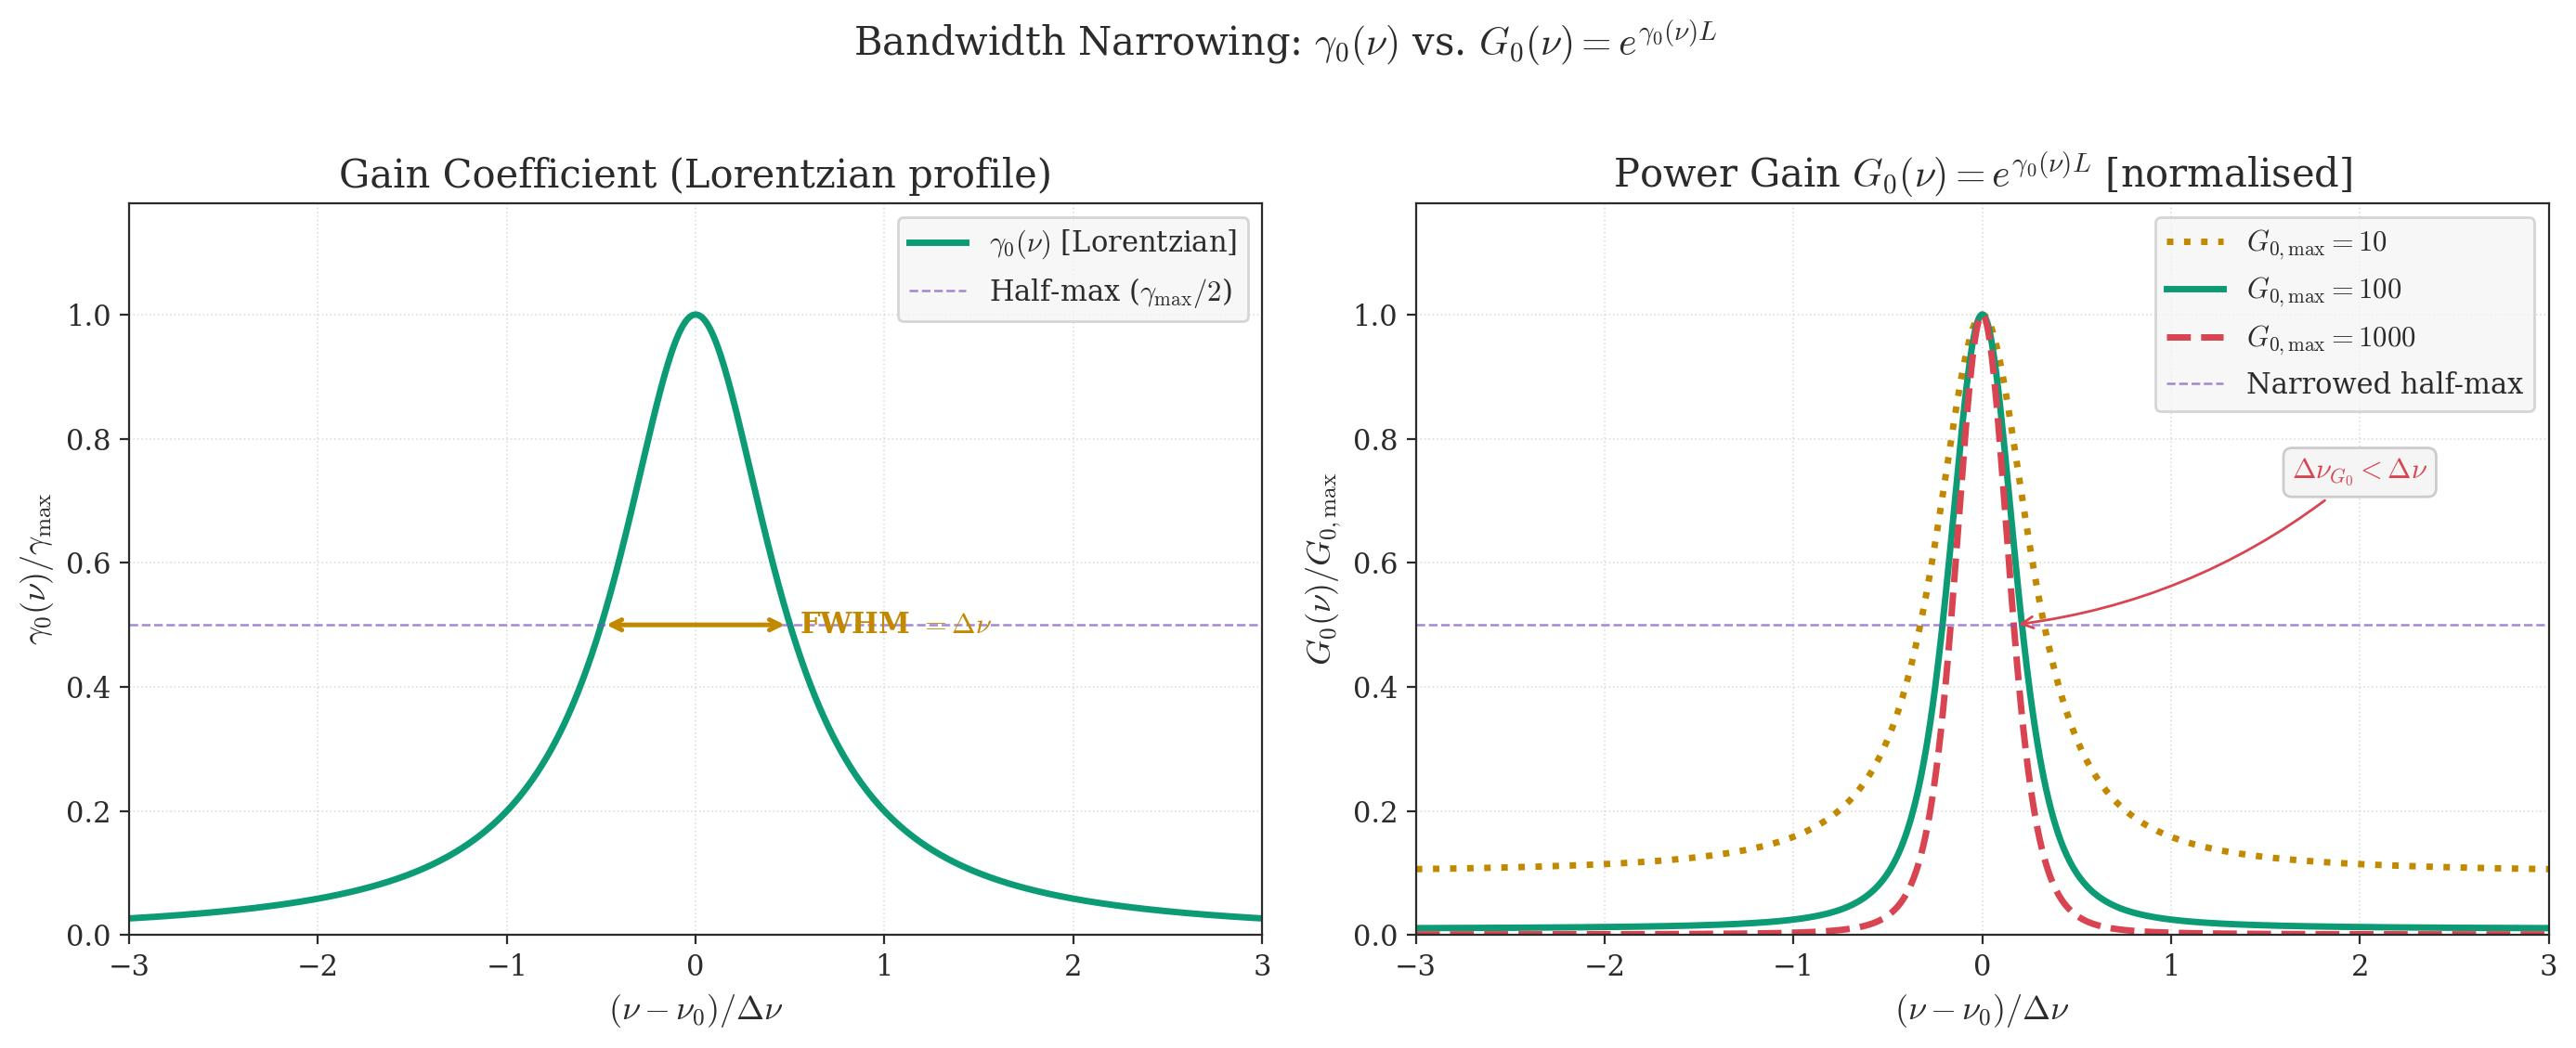
\includegraphics[width=0.7\textwidth]{Figures/Chapter 3/gain_narrowing_output.jpg}
    \caption{Gain Narrowing Factor vs. Output Gain: Demonstrating that massive gain directly destroys signal bandwidth.}
\end{figure}


% ------- NOISE -----------------------------------------------
\subsection{Noise Performance}

The noise performance is the third fundamental parameter of an optical amplifier.  In
an optical amplifier, the dominant noise source is \textbf{amplified spontaneous
emission (ASE)}: spontaneous emission photons emitted into the signal mode get
amplified along with the signal, adding a fluctuating background that degrades the
signal quality.  We now derive the ASE power and the optical signal-to-noise ratio
from first principles.

\subsubsection*{Why Spontaneous Emission Is the Dominant Noise Source}

Spontaneous emission occurs randomly in all directions, with random polarisation, and at random frequencies within the atomic linewidth.
Only a fraction of these spontaneous photons happen to be emitted into the
\emph{same spatial mode} as the signal, and only half of those share the same
\emph{polarisation}.  Those two fractions are what get amplified by the gain medium
and added to the signal — everything else is noise in the wrong direction or wrong
polarisation, and is either lost or filtered out.

\begin{figure}[H]
    \centering
    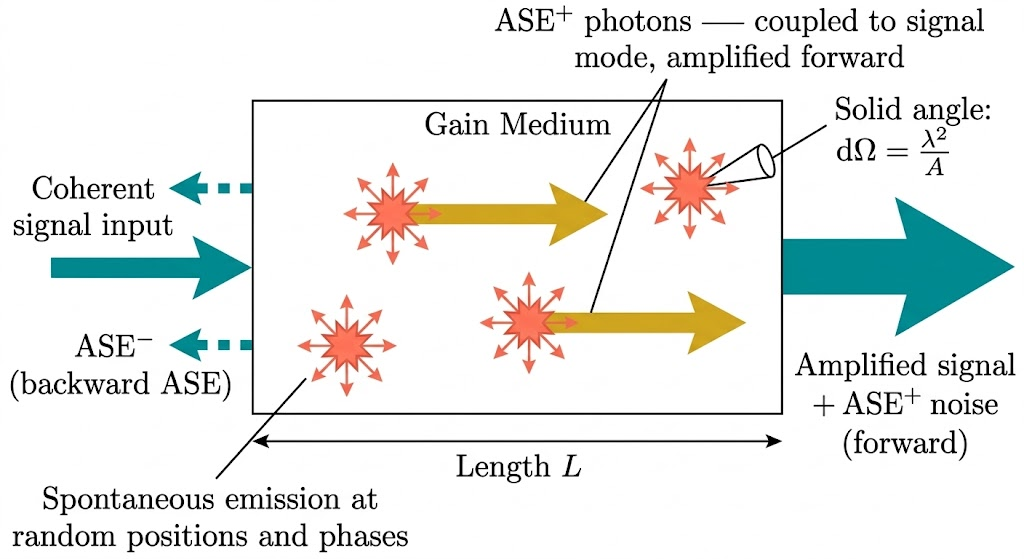
\includegraphics[width=0.8\textwidth]{Figures/Chapter 3/ase_noise.jpg}
    \caption{ASE Noise: Visualizing spontaneous emission creating uncorrelated broadband noise photons ($\text{ASE}^{+}$ and $\text{ASE}^{-}$) travelling collinearly with the amplified signal.}
\end{figure}

\subsubsection*{Step 1: Spontaneous Emission Rate Into a Volume Element}

We start by considering a thin slab of gain medium of cross-sectional area $A$
and thickness $\delta z$.  The rate of spontaneous emission from $N_2$ atoms per
unit volume per unit time per unit frequency interval is:
\begin{equation*}
    \frac{N_2}{\tau_{sp}} \cdot g_{\nu_0}(\nu) \cdot \delta\nu,
\end{equation*}
where $\tau_{sp}$ is the spontaneous emission lifetime, $g_{\nu_0}(\nu)$ is the
normalised lineshape function, and $\delta\nu$ is the frequency bandwidth we are
tracking.  The total spontaneous emission rate (photons per second) from the volume
$A \cdot \delta z$ into bandwidth $\delta\nu$ is therefore:
\begin{equation*}
    \text{Rate} = \frac{N_2}{\tau_{sp}} \cdot g_{\nu_0}(\nu) \cdot \delta\nu
    \cdot A \cdot \delta z.
\end{equation*}

\subsubsection*{Step 2: Fraction Coupled Into the Signal Mode}

These spontaneous photons are emitted isotropically into a total solid angle
of $4\pi$ steradians.  To find the fraction that are emitted into the
\emph{laser beam direction} (i.e., into the signal spatial mode), we use the
concept of the \textbf{laser solid angle}.

The solid angle element in spherical coordinates is:
\begin{equation*}
    d\Omega = \sin\theta\,d\theta\,d\phi,
\end{equation*}
and the total solid angle of a full sphere is:
\begin{equation*}
    \Omega_\text{total} = \int_0^{2\pi}\int_0^{\pi} \sin\theta\,d\theta\,d\phi = 4\pi.
\end{equation*}

For a beam of wavelength $\lambda$ propagating through a medium of cross-sectional
area $A$, diffraction theory tells us that the beam subtends a solid angle:
\begin{equation*}
    d\Omega_\text{laser} = \frac{\lambda^2}{A}.
\end{equation*}
This is the \textbf{laser solid angle} — the solid angle subtended by the single
spatial mode of the laser beam.

The fraction of spontaneous emission coupled into the laser mode is therefore:
\begin{equation*}
    \frac{d\Omega_\text{laser}}{\Omega_\text{total}} = \frac{\lambda^2/A}{4\pi}
    = \frac{\lambda^2}{4\pi A}.
\end{equation*}

\subsubsection*{Step 3: Accounting for Polarisation}

The signal beam has a definite polarisation.  Spontaneous emission is equally
likely to be in any polarisation — on average, only half the spontaneously emitted
power is in the same polarisation as the signal.  This introduces an additional
factor of $1/2$.

To see this more formally: the electric field of a spontaneously emitted photon
can be decomposed into two orthogonal polarisations, $E_x = E_0\cos\theta$ and
$E_y = E_0\sin\theta$, where $\theta$ is uniformly distributed over $[0, 2\pi)$.
The average intensity in the $x$-polarisation is:
\begin{equation*}
    \langle I_x \rangle = E_0^2 \langle \cos^2\theta \rangle
    = E_0^2 \cdot \frac{1}{2\pi}\int_0^{2\pi}\cos^2\theta\,d\theta
    = \frac{E_0^2}{2} = \frac{I}{2}.
\end{equation*}
So only half the intensity is in the signal's polarisation — this factor of $1/2$
is sometimes called the \textbf{Stokes factor}.

\subsubsection*{Step 4: Spontaneous Emission Power Coupled to Signal}

Combining steps 1–3, the spontaneous emission power coupled into the signal mode
(same direction and same polarisation) from the volume element $A \cdot \delta z$
within bandwidth $\delta\nu$ is:
\begin{equation*}
    dP_\text{sp-coupled}
    = \frac{N_2}{\tau_{sp}} \cdot g_{\nu_0}(\nu) \cdot \delta\nu
    \cdot A \cdot \delta z \cdot h\nu
    \cdot \frac{\lambda^2}{4\pi A} \cdot \frac{1}{2}.
\end{equation*}
Simplifying (the area $A$ cancels):
\begin{equation*}
    dP_\text{sp-coupled}
    = \frac{N_2}{\tau_{sp}} \cdot g_{\nu_0}(\nu) \cdot \delta\nu \cdot h\nu
    \cdot \frac{\lambda^2}{8\pi} \cdot \delta z.
\end{equation*}
Dividing by $\delta z$ to get the spontaneous emission power added per unit length:
\begin{equation*}
    \frac{dP_\text{ASE}}{dz}
    = \frac{N_2 h\nu\,\lambda^2}{8\pi\tau_{sp}} \cdot g_{\nu_0}(\nu) \cdot \delta\nu.
\end{equation*}

\subsubsection*{Step 5: Introducing the Spontaneous Emission Factor \texorpdfstring{$n_{sp}$}{n\_sp}}

The cross-section relation $\sigma(\nu) = \frac{\lambda^2}{8\pi\tau_{sp}}\,g_{\nu_0}(\nu)$ and the gain coefficient definition $\gamma = \sigma(N_2 - N_1)$, giving $\sigma = \gamma/(N_2 - N_1)$, let us write:
\begin{equation*}
    \frac{dP_\text{ASE}}{dz}
    = N_2 h\nu \cdot \sigma(\nu) \cdot \delta\nu
    = h\nu\,\delta\nu \cdot \sigma(\nu) \cdot N_2.
\end{equation*}
Physically, we expect the noise power to scale with how fully inverted the medium is: a completely inverted medium (all atoms in $E_2$, none in $E_1$) should produce the minimum possible noise per unit gain, while a weakly inverted medium wastes more of its pump energy on re-absorption. To isolate this quality factor, we multiply and divide the expression by $(N_2 - N_1)$, which lets us group the $\sigma(N_2 - N_1) = \gamma$ term and expose the inversion-quality ratio separately:
\begin{equation*}
    \frac{dP_\text{ASE}}{dz}
    = h\nu\,\delta\nu \cdot \underbrace{\sigma(\nu)(N_2 - N_1)}_{\gamma}
    \cdot \frac{N_2}{N_2 - N_1}.
\end{equation*}
We define the \textbf{spontaneous emission factor} (also called the \textbf{population
inversion factor}):
\begin{keyresult}
\begin{equation}
    n_{sp} = \frac{N_2}{N_2 - N_1}
\end{equation}
\end{keyresult}

where $n_{sp}$ is always $\geq 1$ (since $N_2 \geq N_2 - N_1$ whenever $N_1 \geq 0$),
and approaches 1 only in the limit of complete inversion ($N_1 \to 0$).  It is a
direct measure of how noisy the amplifier is: $n_{sp} = 1$ is the ideal (quantum
noise limited) case, while $n_{sp} \gg 1$ indicates significant noise.

After passing through an optical bandpass filter of bandwidth $B_0$ (which selects
only the frequency band of interest around the signal), the ASE power per unit
length becomes:
\begin{keyresult}
\begin{equation}
    \frac{dP_\text{ASE}}{dz} = \gamma\,n_{sp}\,h\nu\,B_0
\end{equation}
\end{keyresult}

This is the ASE noise power added to the signal beam \emph{per unit length of
amplifier}, after spatial and polarisation filtering.

\subsubsection*{Step 6: Total Power Propagation Equation}

Now we write the total power change equation.  The signal power $P$ increases due
to stimulated emission (gain) and is augmented by ASE noise:
\begin{equation}
    \frac{dP}{dz} = \underbrace{\gamma\,P}_{\text{signal gain}}
    + \underbrace{\gamma\,n_{sp}\,h\nu\,B_0}_{\text{ASE noise}}. \tag{I} 
\end{equation}

To solve this, we assume the small-signal regime ($\gamma = \gamma_0 = $ constant). This is then a first-order linear ODE with constant coefficients. Rearranging:
\begin{equation*}
    \frac{dP}{dz} - \gamma_0\,P = \gamma_0\,n_{sp}\,h\nu\,B_0.
\end{equation*}
The right-hand side is a constant (call it $C = \gamma_0 n_{sp} h\nu B_0$).  The
general solution to $P' - \gamma_0 P = C$ is the sum of the homogeneous solution
$P_h = P(0)\,e^{\gamma_0 z}$ and a particular solution $P_p = -C/\gamma_0 = -n_{sp}
h\nu B_0$.  Applying the boundary condition $P(0) = P_\text{in}$:
\begin{equation*}
    P(z) = \left(P_\text{in} + n_{sp}h\nu B_0\right)e^{\gamma_0 z} - n_{sp}h\nu B_0.
\end{equation*}
Evaluating at $z = L$ and using $G_0 = e^{\gamma_0 L}$:
\begin{keyresult}
\begin{equation}
    P(L) = G_0\,P_\text{in} + n_{sp}\,h\nu\,B_0\,(G_0 - 1)
\end{equation}
\end{keyresult}

This is a beautiful and important result.  The output power has two terms:
\begin{itemize}
    \item $G_0\,P_\text{in}$: the amplified signal — this is the desired output.
    \item $n_{sp}\,h\nu\,B_0\,(G_0 - 1)$: the ASE noise power added by the
    amplifier.  Notice that this term vanishes ($G_0 = 1$) when there is no gain,
    and grows with $G_0$ — more gain means more noise.
\end{itemize}

\subsubsection*{Step 7: Optical Signal-to-Noise Ratio}

The \textbf{optical signal-to-noise ratio (OSNR)} of the amplifier output is
defined as the ratio of amplified signal power to ASE noise power:
\begin{equation*}
    \text{OSNR} = \frac{G_0\,P_\text{in}}{n_{sp}\,h\nu\,B_0\,(G_0 - 1)}.
\end{equation*}
In the practically relevant limit of high gain ($G_0 \gg 1$, so $G_0 - 1 \approx
G_0$):
\begin{keyresult}
\begin{equation}
    \text{OSNR} \approx \frac{P_\text{in}}{n_{sp}\,h\nu\,B_0}
\end{equation}
\end{keyresult}

The OSNR is \emph{independent of the gain} $G_0$ in the high-gain limit — a remarkable and practically decisive result. No matter how large the gain is, the OSNR saturates at $P_\text{in}/(n_{sp}h\nu B_0)$. The only levers available to improve the OSNR are: increasing the input signal power $P_\text{in}$, achieving a more complete population inversion (reducing $n_{sp}$ toward 1 as $N_1 \to 0$), or narrowing the filter bandwidth $B_0$ (at the cost of signal bandwidth).


Analyzing the output floor, the undeniable dominant noise source in any optical amplifier is ASE. These are just rogue spontaneous emission photons that statistically happen to couple perfectly into the signal mode and steal amplification. Only the tiny fraction aligning with the signal's exact direction and true polarization manages to matter. That fraction piles up as the ASE power term $n_{sp}h\nu B_0(G_0-1)$ on the backend, hard-locking the high-gain optical SNR strictly at $P_\text{in}/(n_{sp}h\nu B_0)$, entirely immune to further gain. The spontaneous emission factor $n_{sp} = N_2/(N_2-N_1) \geq 1$ acts as the ultimate figure of merit for the amplifier's internal noise hygiene — an $N_1$ starved of atoms ($n_{sp} \to 1$) makes for the cleanest possible amplifier.

\begin{figure}[H]
    \centering
    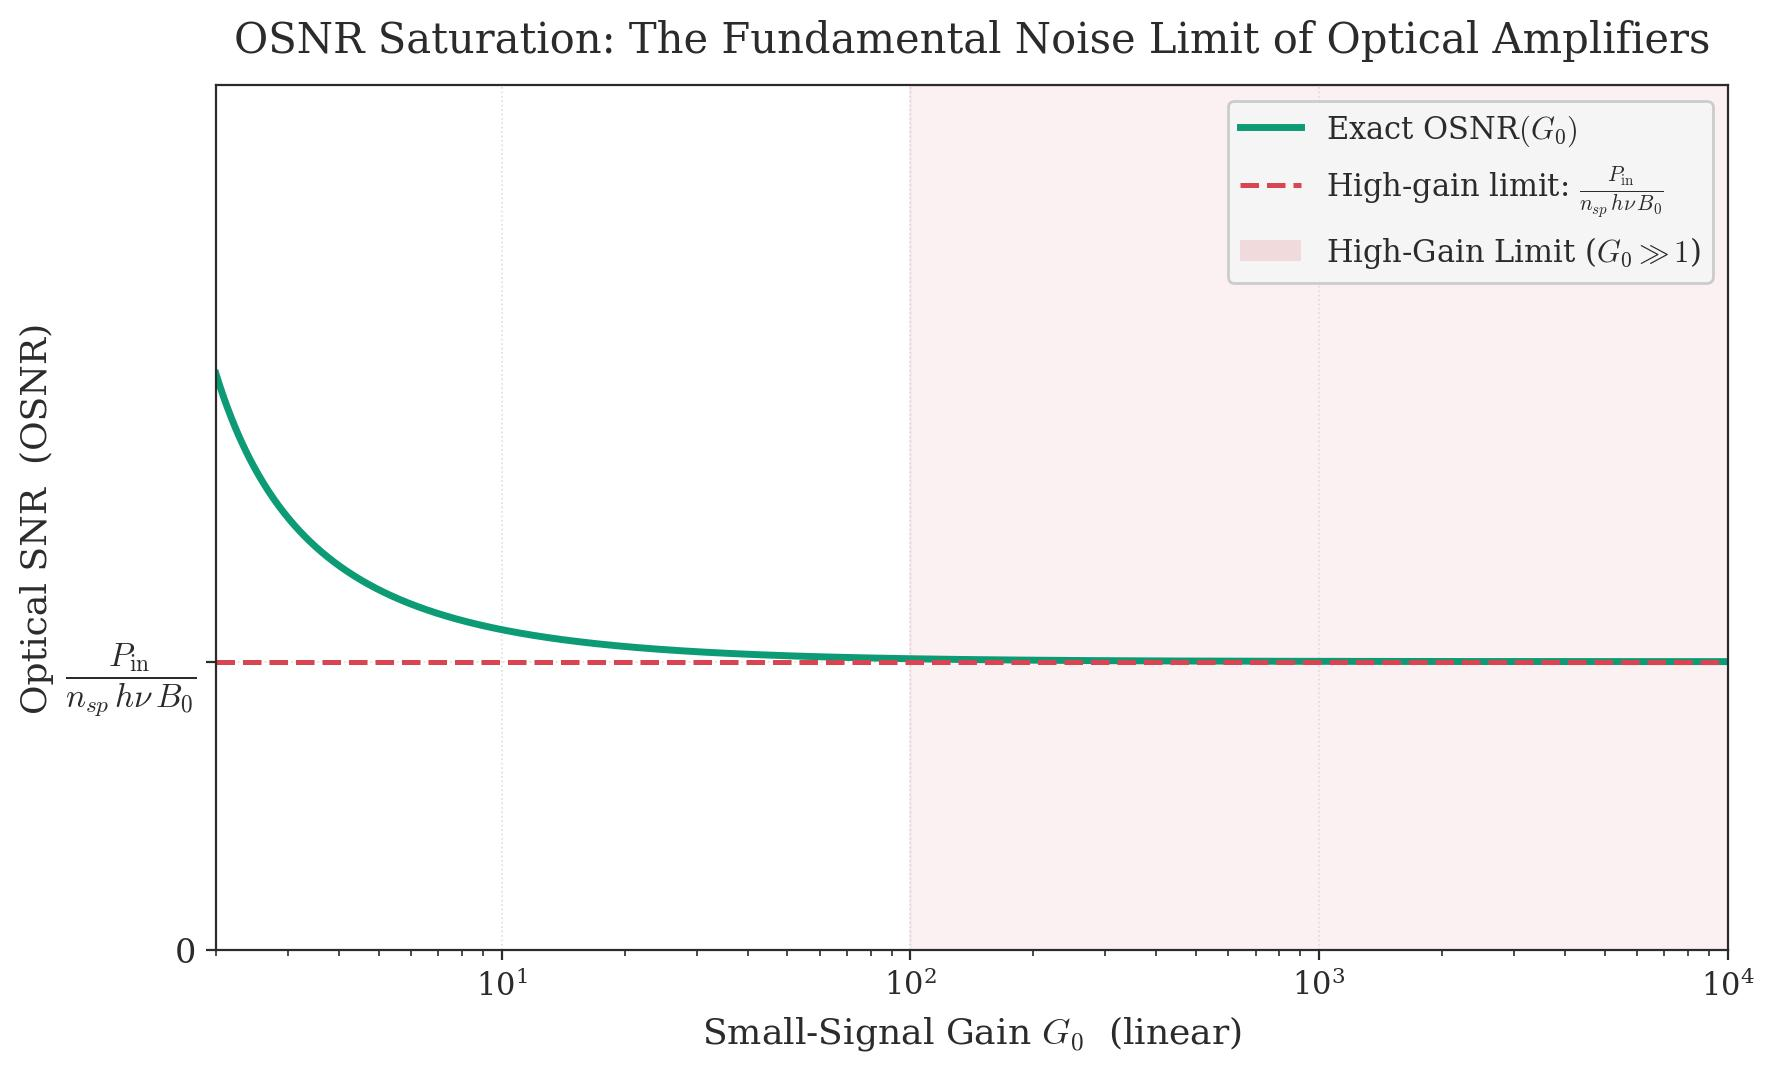
\includegraphics[width=0.7\textwidth]{Figures/Chapter 3/osnr_asymptote.jpg}
    \caption{OSNR Asymptote: The fundamental noise limit of optical amplifiers at high linear gain values.}
\end{figure}
% =============================================================
\section{Case Study: The Erbium-Doped Fibre Amplifier (EDFA)}
% =============================================================
\subsection{What is an EDFA?}
The Erbium-Doped Fibre Amplifier (EDFA) is the canonical real-world application of the three-level laser system we just derived. It is a Travelling-Wave Amplifier (TWA) built directly inside an optical fibre, amplifying light \emph{without} ever converting it to an electrical signal first.

As the name implies, "Erbium Doped" simply means the native silica glass fiber core (the Host) has been infused with Erbium ions ($\mathrm{Er}^{3+}$) during manufacturing.

\subsection{Working Principle (A Step-By-Step Sequence)}
To master how the EDFA works, we must walk through its sequence chronologically:
\begin{enumerate}
  \item \textbf{Signal Light Enters:} A weak optical signal carrying internet information enters the erbium-doped fiber section. The wavelength is typically near $\lambda = \SI{1550}{nm}$ because this is the global minimum loss window for silica host glass.
  \item \textbf{Pump Laser Creates Inversion:} A separate, higher-energy laser (usually permanently shining at $\lambda = \SI{980}{nm}$) pumps energy rapidly down the fiber alongside the signal. This $\SI{980}{nm}$ light violently excites the sluggish $\mathrm{Er}^{3+}$ ions, ripping them from their ground state $E_1$ up into a metastable (slow-to-relax, meaning long $\tau_t$) upper state $E_2$. This pump action sustains the highly non-natural \textbf{Population Inversion} ($N_2 > N_1$) we mathematically proved was required for gain!
  \item \textbf{Stimulated Emission Triggers:} When the weak $\SI{1550}{nm}$ signal wave smoothly passes through this excited cloud of erbium ions, the electric field of the signal interacts with the inversion. It forces the ions to quickly release their stored top-level energy. The ions instantly drop down to $E_1$ and release photons that are exact engineered "clones" of the incident signal. 
  \item \textbf{Output Signal Exits:} Because the cloned photons perfectly match the original wave's frequency and phase, they constructively add to the signal envelope. The light exits the fiber massively stronger ($10 - 30$ dB gain), yet containing the exact same pristine digital data packet ($P_{\text{out}} \gg P_{\text{in}}$).
\end{enumerate}

\begin{figure}[H]
    \centering
    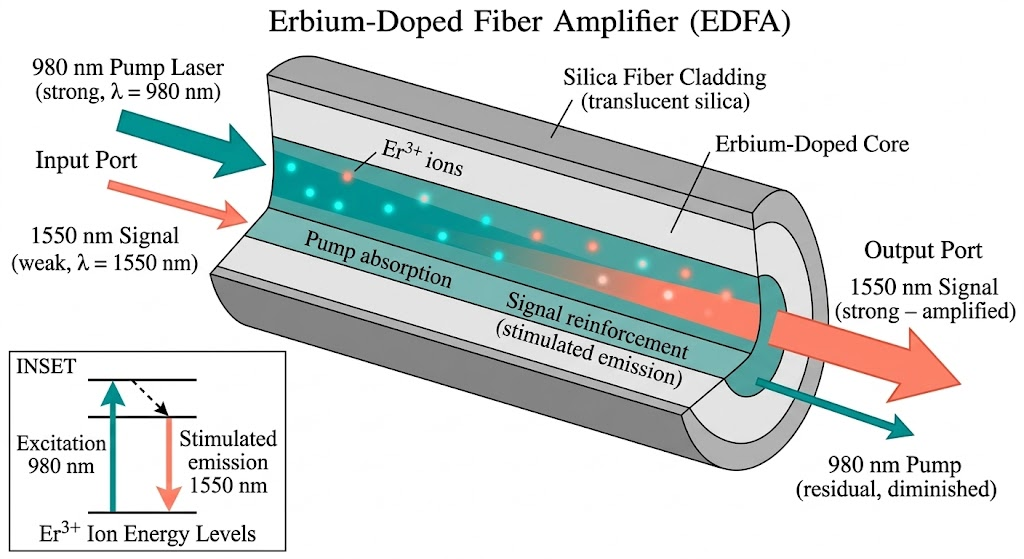
\includegraphics[width=0.7\textwidth]{Figures/Chapter 3/edfa_architecture.jpg}
    \caption{The Erbium-Doped Fiber Amplifier (EDFA): A masterclass application synthesizing all principles—population inversion via 980 nm pumping, metastable persistence, and massive 1550 nm single-pass signal amplification driven entirely by stimulated emission within a solid state fiber core.}
\end{figure}

So, at its core, the EDFA wields a secondary 980 nm pump laser explicitly to force and lock a massive population inversion across the embedded Erbium ions. This brilliantly sets the kinetic stage for a weak 1550 nm passing signal to linearly drain that stored atomic energy precisely via stimulated emission, allowing it to exit the fiber continuously and heavily amplified.



% =============================================================

\section{Summary and Looking Ahead}

% =============================================================



We have now built a complete picture of optical amplification:



\begin{enumerate}

  \item We derived the small-signal propagation equation $d\Phi/dz = \gamma_0\,\Phi$ by balancing photon creation (stimulated emission) and destruction (absorption) in a differential element of the medium.

  \item We showed that gain ($\gamma_0 > 0$) requires $N_2 > N_1$ --- \textbf{population inversion} --- which is achieved by a pump before the signal enters.

  \item We wrote the \textbf{rate equations} for $N_2$ and $N_1$ with a single pump rate $R$ transferring atoms from the ground state $E_1$ into $E_2$ via the fast pump level $E_3$.

  \item We proved algebraically that a \textbf{two-level laser is impossible} ($N_2/N_1 < 1$ always), and showed that a three-level (or four-level) architecture separates the pump and lasing transitions, breaking the symmetry and enabling inversion.

  \item We worked through the \textbf{three-level laser system} explicitly, deriving $N_0$, $\Phi_s$, and the threshold pump rate for constant-rate and optical pumping models --- the direct foundation for the EDFA.

  \item Once a signal is present, the gain saturates: $\gamma = \gamma_0/(1+P/P_s)$ in the general (homogeneous) case.

  \item The amplifier's \textbf{gain} is $G_0 = e^{\gamma_0 L}$ in the small-signal limit and decreases with input power in the general case.

  \item The amplifier's \textbf{bandwidth} is narrower than the atomic linewidth $\Delta\nu$ whenever $G_{0,\max} > 4$ (bandwidth narrowing), with the precise FWHM given by $\Delta\nu_{G_0} = \Delta\nu\sqrt{\ln(G_{0,\max})/\ln(G_{0,\max}/2)-1}$.

  \item The amplifier's \textbf{noise} is dominated by ASE, yielding the output power $P(L) = G_0 P_\text{in} + n_{sp}h\nu B_0(G_0-1)$ and a high-gain OSNR of $P_\text{in}/(n_{sp}h\nu B_0)$, independent of gain.

  \item For inhomogeneously broadened media, the gain saturates as $\gamma_0/\sqrt{1+P/P_s}$, requiring $\sim 3P_s$ to halve the gain rather than $P_s$.

  \item We decomposed the polarisation of a doped host medium into \textbf{host} and \textbf{transition} contributions, showing that the tiny complex $\chi_\text{trans}$ acts as a perturbation on the host refractive index, governing both the phase shift and the gain.

  \item We applied all of the above in the \textbf{EDFA} --- the Erbium-Doped Fiber Amplifier --- the most important practical realisation of single-pass optical amplification in modern telecommunications.

\end{enumerate}



Now that we fully understand the concept of optical amplification and the physics of the gain medium, we are ready to place this gain medium inside a resonant cavity and study how feedback turns a travelling-wave amplifier into a \textbf{laser oscillator}. The next chapter will derive the conditions for self-sustained oscillation, the allowed mode frequencies, the threshold pump rate, and the output power of the laser.
